%% 
%% Copyright 2019-2021 Elsevier Ltd
%% 
%% This file is part of the 'CAS Bundle'.
%% --------------------------------------
%% 
%% It may be distributed under the conditions of the LaTeX Project Public
%% License, either version 1.2 of this license or (at your option) any
%% later version.  The latest version of this license is in
%%    http://www.latex-project.org/lppl.txt
%% and version 1.2 or later is part of all distributions of LaTeX
%% version 1999/12/01 or later.
%% 
%% The list of all files belonging to the 'CAS Bundle' is
%% given in the file `manifest.txt'.
%% 
%% Template article for cas-sc documentclass for 
%% single column output.

% Document Class
\documentclass[a4paper,fleqn]{cas-sc}

% Packages
\usepackage[authoryear,longnamesfirst]{natbib}

%Package to hold figure in position
\usepackage{placeins}

%Author macros
\def\tsc#1{\csdef{#1}{\textsc{\lowercase{#1}}\xspace}}
\tsc{WGM}
\tsc{QE}

\begin{document}
\let\WriteBookmarks\relax
\def\floatpagepagefraction{1}
\def\textpagefraction{.001}

% Short title
\shorttitle{Numerical analysis of the rock deformation in twin tunnels with transverse galleries}    

% Short author
\shortauthors{Quevedo et al.}  

% Main title of the paper
\title [mode = title]{Numerical analysis of the rock deformation in twin tunnels with transverse galleries considering plasticity and time-dependent constitutive models}  

% First author
\author[1]{Quevedo, F. P. M.}[style = chinese, orcid = 0000-0003-4171-1696]
\cormark[1] 					
\cortext[cor1]{Corresponding author.}
\ead{motta.quevedo@ufrgs.br}
\ead[url]{https://www.researchgate.net/profile/Felipe-Pinto-Da-Motta-Quevedo}

% Second author
\author[1]{Colombo, C. A. M. M.}[style=chinese]
\ead{ca-colombo@hotmail.com}
\ead[url]{http://lattes.cnpq.br/4919388217690564}

% Third author
\author[1]{Bernaud, D.}[style=chinese, orcid=0000-0001-6365-3269]
\ead{denise.bernaud@ufrgs.br}
\ead[url]{http://lattes.cnpq.br/2809615143819128}

% Four author
\author[1]{Maghous, S.}[style=chinese, orcid=0000-0002-1123-3411]
\ead{samir.maghous@ufrgs.br}
\ead[url]{https://www.researchgate.net/profile/Samir-Maghous}

% Afilliation
\affiliation[1]{organization={Federal University of Rio Grande do Sul},
	addressline={Av. Osvaldo Aranha, 99}, 
	city={Porto Alegre},
	postcode={90.035-190}, 
	state={RS},
	country={Brazil}}

% Mathematical Symbols
\newcommand{\dgds}{\boldsymbol{g_\sigma}}
\newcommand{\Dll}{\boldsymbol{D}}
\newcommand{\Dllmod}{\boldsymbol{D^{*}}}
\newcommand{\Dllepvp}{\boldsymbol{D}^{epvp}}
\newcommand{\dstrain}{\boldsymbol{\dot{\varepsilon}}}
\newcommand{\dstraine}{\boldsymbol{\dot{\varepsilon}}^{e}}
\newcommand{\dstrainp}{\boldsymbol{\dot{\varepsilon}}^{p}}
\newcommand{\dstrainv}{\boldsymbol{\dot{\varepsilon}}^{vp}}
\newcommand{\straineqp}{\bar \varepsilon^p}
\newcommand{\dstrainsh}{\boldsymbol{\dot{\varepsilon}}^{sh}}
\newcommand{\dstraincr}{\boldsymbol{\dot{\varepsilon}}^{cr}}
\newcommand{\dstress}{\boldsymbol{\dot{\sigma}}}
\newcommand{\onell}{\boldsymbol{1}}
\newcommand{\strain}{\boldsymbol{\varepsilon}}
\newcommand{\straincr}{\boldsymbol{\varepsilon}^{cr}}
\newcommand{\straine}{\boldsymbol{\varepsilon}^{e}}
\newcommand{\strainp}{\boldsymbol{\varepsilon}^{p}}
\newcommand{\strainsh}{\boldsymbol{\varepsilon}^{sh}}
\newcommand{\strainshCEB}{\varepsilon_{sh}}
\newcommand{\strainvp}{\boldsymbol{\varepsilon}^{vp}}
\newcommand{\stress}{\boldsymbol{\sigma}}
\newcommand{\zerol}{\boldsymbol 0}

% Here goes the abstract
\begin{abstract}
Resorting a three-dimensional finite element analysis, this paper investigates the instantaneous and long-term implications induced by the time-dependent constitutive behavior of constituents on the convergence profile of twin tunnels linked with transverse galleries. Several constitutive models for rock mass mechanical behavior are examined at the material level, encompassing elastoplasticity, viscoplasticity, or coupled elastoplasticity-viscoplasticity frameworks. Plasticity state equations are based on a Drucker-Prager yield surface with an associated flow rule, while the viscoplasticity formulation relies on the Perzyna model with a Drucker-Prager flow surface. Tunnel lining behavior is modeled using either elastic or viscoelastic constitutive models. The viscoelastic behavior is described by a Generalized Kelvin rheological model based on Bazant and Prassanann's Solidification Theory, with model parameters derived from CEB-FIP MC90 formulations. From a computational viewpoint, the deactivation-activation method is employed to simulate the excavation process and lining installation. The accuracy of finite element predictions is assessed through comparisons with available analytical solutions formulated in a simplified setting for the twin tunnels' configuration. A parametric study delves into the mutual interaction induced by tunnels proximity, emphasizing the crucial role of concrete lining stiffness in twin tunnels' deformation. Numerical simulations indicate a highly localized influence of a transverse gallery on twin tunnels deformation, extending up to four radii from each side of the gallery axis. Finally, the paper investigates the effects of twin tunnels proximity and those induced by an interconnecting gallery on the instantaneous and long-term convergence of tunnels, contrasting these outcomes with the convergence of a single tunnel.
\end{abstract}

% Use if graphical abstract is present
\begin{graphicalabstract}
	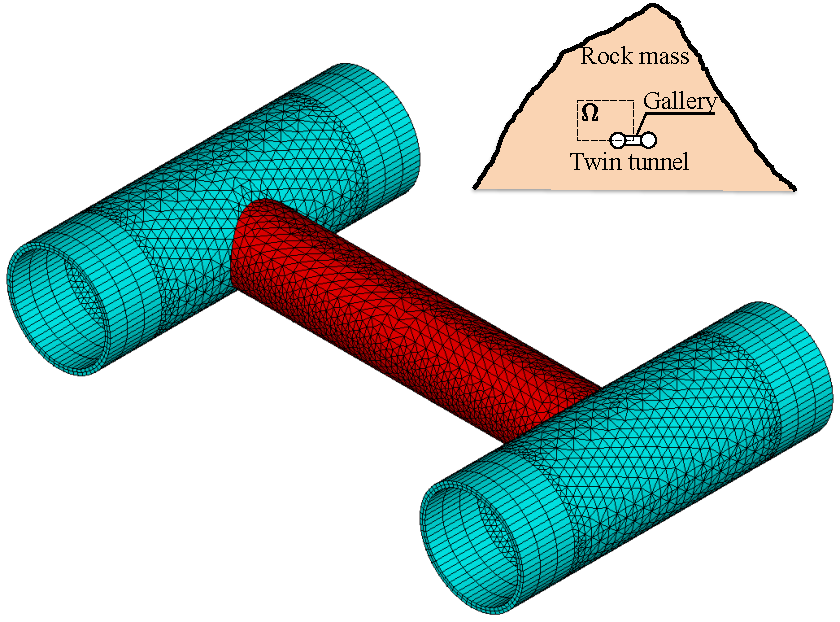
\includegraphics[scale=1]{graphical_abstract.pdf}
\end{graphicalabstract}

% Research highlights
\begin{highlights}
	\item The stiffness of the lining restricting viscous effects in the interaction of tunnels
	\item Interaction between the tunnels becomes significant at a span distance of 4 radii
	\item The viscous of the concrete lining can be important in the tunnel convergence
	\item The effect of the gallery extends into the tunnel up to 4 radii from its axis
	\item The proximity of the tunnels induces the ovalization of the tunnel wall 
\end{highlights}

% Keywords
\begin{keywords}
twin tunnels \sep transverse gallery \sep elastoplasticity-viscoplasticity coupling
\sep viscoelastic lining \sep finite element method
\end{keywords}

\maketitle

\section{Introduction}\label{}

Many design methods often focus on single tunnels, but twin tunnels are a common occurrence. The interaction between tunnels can be significant, especially when the spacing between them is minimal. Additionally, many twin tunnels incorporate transverse galleries, introducing a localized effect on displacements and stresses. Also, the rheological behavior of the rock mass and lining plays a crucial role in how stress and displacements fields evolve over time. Some recent studies on deep twin tunnels can be found at [\citenum{Spyridis2015}, \citenum{Chen2019}, \citenum{Fortsakis2021}, \citenum{chortis2021a},\citenum{chortis2021b}, \citenum{GUO2021}, \citenum{chortis2023a}, \citenum{chortis2023b}].

Chortis and Kavvadas [\citenum{chortis2021a}] considered the calculation of the axial forces acting on the primary support in the intersection zone before, during, and after the construction of a perpendicular tunnel intersection. The results of the analysis indicated that the zone of influence extends approximately two diameters from the main tunnel to each side from the center of the intersection and that the interaction effects are practically eliminated when they exceed this influence zone. 

In another study, Chortis and Kavvadas [\citenum{chortis2021b}] carried out parametric 3D finite element analyses to verify the interaction between deep twin tunnel, with circular and non-circular cross-section, supported by a shotcrete elastic linear lining. Was considering the rock mass with linear elastic behavior and perfectly plastic, with Mohr-Coulumb failure criteria. The study investigates the axial forces that develop in the primary lining of the twin tunnels as a function of the main geometric and geomaterial parameters, but without considering the potential time-dependent deformations (creep effect) that occur in some types of rock masses.

Chen et al. [\citenum{Chen2019}], through analytical solutions in elasticity using complex variables, Fourier transformation, and the alternating Schwarz method, demonstrate that the mutual interaction between twin tunnels disappears if the spacing between the tunnels is greater than six times the tunnel radius. The lining effectively reduces the stress concentration, especially at high lateral stress coefficients.

Guo et al. [\citenum{GUO2021}] develop an elastic analytical solution for the stress field around twin circular tunnels with hydrostatic pressure using the complex variable and the superposition principle. They found that stress concentration in tunnel wall increased as the distance between the parallel tunnels decreased and the supporting pressure leads to the radial stress increasing and the tangential stress decreasing.

Ma et al. [\citenum{MA2020}] proposed an analytical method, verified by a numerical solution using FLAC3D software for determining the plastic zones around deep circular twin tunnels without linings, restricting themselves where there is no overlap between the two plastic zones. In this case, the authors adopted the elastoplastic perfectly constitutive model for the homogeneous and isotropic rock mass, with the Mohr-Coulomb criterion. Also carried out parametric studies to understand the influence of the distance between the twin tunnels, cohesion, the angle of internal friction, and the vertical and horizontal initial stresses acting on the shape and depth of the plastic zones. These authors stated that the plastic zone around the tunnel provides a relevant theoretical basis for defining and designing the support. In that respect, an excessive plastic zone would significantly affect the stability and functionality of a tunnel. Reducing the extension of the plastic zone around tunnels is, therefore, of great importance in engineering tunnel design projects.

Using parametric three-dimensional numerical analyses, Chortis and Kavvadas [\citenum{chortis2023a}, \citenum{chortis2023b}] investigated the effect of building a transverse tunnel that intersected deep twin tunnels perpendicularly, focusing the study on the axial forces and the circumferential and longitudinal bending moments acting on the primary support of the intersection regions, respectively. According to the authors, the potential interaction between deep twin tunnels lined with shotcrete must be taken into account, especially when the distance between them is less than or equal to twice their diameter.

According to Fortsakis [\citenum{Fortsakis2021}], in a realistic construction context, twin tunnels are excavated and supported with a delay, so that the second tunnel is usually built after the first one has advanced enough to maintain a longitudinal separation distance between the faces. The advance of the subsequent tunnel mobilizes the redistribution of stresses and deformations in the zone between the tunnels, resulting in additional loading of the preceding tunnel.

As for transverse tunnels, these are generally built far enough behind the advanced face of the main tunnel to ensure that their excavation has virtually no effect during the construction of the junction tunnel [\citenum{chortis2021a}]. The interaction at the intersection, between the main tunnel and the transverse tunnel, significantly modifies the stress state of the primary support and that of the surrounding rock mass in these areas, compared to that of the singular tunnel, making three-dimensional finite element analyses essential for developing a realistic and safe design for tunnel junctions [\citenum{Spyridis2015}].

During the construction of the transverse tunnel, the surrounding rock mass is subjected to a redistribution of stresses, causing an additional load on the main tunnel, precisely in the intersection zone. If these additional loads exceed the load capacity of the primary support of the main tunnel, a potentially unstable region can develop, leading to failure, especially in adverse geotechnical conditions [\citenum{chortis2021a}].

While the simulation of tunnel convergence in single tunnels has been widely investigated and reported in published literature, few works have addressed the computational evaluation of deformation in twin tunnels. Less attention has been dedicated to assessing the mutual mechanical interaction induced by the excavation of the transverse gallery connecting the twin tunnels. 

In this context, the main contributions of this paper may be summarized at both the material and tunnel analysis levels. At the material level, the constitutive state equations of the rock mass are formulated within the framework of coupled plasticity-viscoplasticity, which is relevant for clayey rocks. Such a framework allows capturing the irreversible instantaneous tunnel response (plasticity) as well as the delayed irreversible response (viscoplasticity).  As regards the mechanical behavior of concrete material defining the lining, which is classically modeled through linear elastic relationships, the present analysis considers an aging viscoelastic rheological model relying upon the Bažant and Prasannan Solidification theory [\citenum{bazant:1989a,bazant:1989b}]. At the structure analysis level, the simulation of deformation in the highly interacting material system components (namely, rock mass and lining), resulting from the excavation process of twin tunnels and transverse gallery, is handled using finite element simulations performed in a three-dimensional setting. From the computational viewpoint, the constitutive models formulated for the rock mass and lining constituent are implemented into the same software utilizing the USERMAT customization tool of ANSYS standard software, together with the related numerical integration schemes.  In this context, the finite element analysis specifically investigates the three-dimensional interaction induced by the construction process, twin tunnels proximity, and the presence of the transverse gallery. 

\section{Fundamental assumptions}\label{}

The basic assumptions of the constitutive and computational modeling, as well as related limitations, are summarized as follows:

\begin{enumerate}[(a)]
	\item Only the configuration of deep tunnels shall be considered in the subsequent analysis, thus neglecting deformations caused by surface loads and settlements arising from the excavation process;

	\item Although material heterogeneity and behavior anisotropy are inherent features of soils and rocks, the rock mass is modeled throughout the paper as a homogeneous and isotropic continuous medium. At the scale adopted for tunnel modeling (macroscopic scale), this assumption means in particular that the possible micro-heterogeneities, such isotropic distributions of joints or cracks present at the finer scale, are accounted for in the homogenized behavior by means of a preliminary homogenization process (e.g., [\citenum{nemat1993}, \citenum{deude2002}, \citenum{deBuhan2002}, \citenum{Marmier2007}, \citenum{Aguiar2023}]). Clearly enough, the framework of continuum modeling adopted in the paper would reveal questionable when the rock mass is cut by a few macro-scale fracture joints;  
	
	\item The rock mass is phenomenologically modeled using an elastoplastic-viscoplastic rheological law to capture instantaneous and long-term responses. This approach disregards the aspect connected temperature gradients, water flow, and poromechanics coupling;

	\item Despite the complexity of the stress distribution prevailing in the rock mass before the process of tunnel excavation, which is mainly affected by the geological history, the present study assumes a geostatic initial stress reflected by an isotropic state of stress.

	\item Twin tunnels are often designed considering a time gap between excavation fronts. However, the finite element simulations assume synchronous excavation steps to ensure symmetry conditions.

	\item The simulation excavation processes are curried out assuming a constant tunnel advancement rate (i.e., constant excavation speed), together with a constant thickness of concrete lining.
	
	\item Effects of temperature and humidity that may affect the viscoelastic behaviour of concrete lining are disregarded.
	
	\item Perfect bonding is assumed at the interface between concrete lining and the rock mas.

	\item The framework of infinitesimal strain analysis, together with quasi-static evolutions, is adopted in the paper. In particular, dynamic excitations and related inertial forces, such as those induced, for instance, by earthquakes or explosions, shall not be considered in the numerical analysis.
	
\end{enumerate}

\section{Constitutive Model of the Rock Material}\label{}



An elastoplastic-viscoplastic constitutive model is formulated and implemented in ANSYS using the UPF/USERMAT customization tool [\citenum{ANSYS:2013b}] to simulate the rock mass. This model assumes importance when conventional models like elastoplasticity or viscoplasticity are inadequate in describing material behavior. This is particularly important in clay rock mass such as those illustrated by Rousset for radioactive waste repositories [\citenum{rousset1988}]. Viscoplasticity models are unable to account the instantaneous plasticization that may arise during tunnel excavation. On the other hand, elastoplastic models fail to capture the temporal evolution of deformations. The elastoplastic-viscoplastic model is formulated based on a serial association of the elastoplastic and viscoplastic constitutive models. The local strain rate $\dstrain$ is split into three contributions $\dstrain = \dstraine + \dstrainp + \dstrainv$, and the constitutive relationships are therefore expressed as:
\begin{equation} \label{eq_constitutive_relationship_epvp}
	\dstress = \Dll : \dstraine = \Dll : (\dstrain - \dstrainp - \dstrainv),\;
\end{equation}
where $\dstress$ denotes the rate of the local Cauchy stress tensor and $\dstraine$, $\dstrainp$, $\dstrainv$, represent the elastic, plastic and viscoplastic strain rate, respectively and $\Dll$ denote the fourth-order isotropic elastic linear constitutive tensor. The one-dimensional representation in Fig.~\ref{reological_scheme} shows this association. 
\begin{figure}[h!]
	\centering
	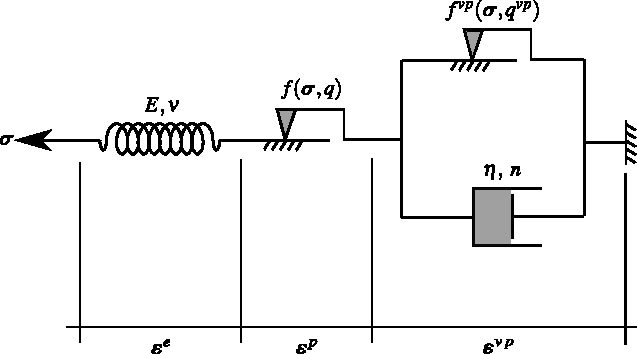
\includegraphics[scale=1]{Rheological representation.pdf}
	\caption{Rheological representation of the elastoplastic-viscoplastic model.}
	\label{reological_scheme}
\end{figure}
In this model is used a Drucker-Prager plastic flow surface given by
\begin{equation}
	\label{eq:f_Drucker_Prager}
	f(\stress,q) = f(I_1,J_2,q) = \beta_1 I_1 +\beta_2 \sqrt{J_2}-q(\alpha),
\end{equation}
which $I_1$ is the first invariant of the stress tensor, $J_2$ the second invariant of the deviator tensor and $\beta_1, \beta_2$ and $q(\alpha)$ are strength parameters related to the friction angle $\phi$ and cohesion $c(\alpha)$, respectively. In the present model Drucker-Prager surface been inner of the Mohr-Coulomb surface [\citenum{bernaud1991}], that is,
\begin{equation}
	\label{eq:f_DP_inscrita_MC}
	\beta_1 = \dfrac{(k-1)}{3}, ~~~ \beta_2 = \dfrac{(2k+1)}{\sqrt{3}}, ~~~
	q(\alpha) = 2\sqrt{k}~c(\alpha),
\end{equation}
where $k = (1+\sin{\phi})/(1-\sin{\phi})$. The internal variable $\alpha$ is the equivalent plastic strain $\straineqp$ used to simulate strain hardening/softening phenomena. However, for this study, we adopt perfect plasticity, meaning that c is a constant. For the viscoplasticity surface $f^{vp}$ the same surface is empolyed, but with $\phi^{vp}$ in $\beta_1$ and $\beta_2$, and $q^{vp} = 2\sqrt{k^{vp}}-c^{vp}$ where $k^{vp} = (1+\sin{\phi^{vp}})/(1-\sin{\phi^{vp}})$ and $c^{vp}$ is a constant, i.e., perfect viscoplasticity. 
The plastic flow rule is given by:
\begin{equation}
	\label{eq_plastic_flow}
	\dot \strainp = \left\{ 
	\begin{array}{ll} 
		\dot \lambda \dfrac{\partial g}{\partial \stress} &  \text{for } f > 0 \\ 
		\zerol, & \text{for } f \le 0 \\
	\end{array}\right.,
\end{equation}
where $\dot \lambda$ is the plasticity multiplier and $g$ is a potential flow function analogous to $f$ used to simulate the volume dilatation during the evolution of plastic deformations. However, for this analysis, was used associated plasticity, i.e., $g=f$. The plastic multiplier is obtained through the consistency condition $\dot f = 0$. Numerical details of this implementation can be found in [\citenum{quevedo2022b}]. For viscoplastic flow rule we have,
\begin{equation}
	\label{eq_viscoplastic_flow}
	\dstrainv = \dot \lambda^{vp} \dfrac{\partial f^{vp}}{\partial \stress}
\end{equation}
In contrast to the plastic multiplier, the viscoplastic multiplier $\lambda^{vp}$ is independent of a consistency condition. As a result, its expression is explicit. For this study, we utilize the Perzyna model [\citenum{perzyna1966}] as follows:
\begin{equation} \label{eq_perzyna_model}
	\dot \lambda^{vp} = \dfrac{\Phi(\stress,q^{vp})}{\eta}~~~\text{and}~~~\Phi = \left\langle  \dfrac{f^{vp}(\stress,q^{vp})}{f_0} \right\rangle^n, \,
\end{equation} where $\Phi$ is the overstress function, $\eta$ is the dynamic viscosity constant, $n$ is the dimensionless parameter that gives the form of the power law, $f_0$ a parameter conveniently adopted and $\left\langle * \right\rangle$ is the McCauley function which is $0$ when $* <0$ , i.e. viscoplastic flow will only occur when the overstress function is positive.

In this coupled model, when $\phi=\phi^{vp}$, cohesion entirely controls the evolution of local mechanical fields. Specifically, when  $c \rightarrow \infty$ and $c^{vp} \rightarrow \infty$, the system achieves a purely elastic solution. The solution becomes purely elastoviscoplastic with $c \rightarrow \infty$, while a pure elastoplastic solution emerges with $c^{vp} \rightarrow \infty$. In coupled analysis, we have adopted $c^{vp} < c$, allowing the viscoplastic domain to occur without plasticity. However, in the presence of plasticity, viscous effects become inevitable. Fig.~\ref{epvpdomains} illustrates these domains in principal stress space.
\begin{figure}[h!]
	\centering
	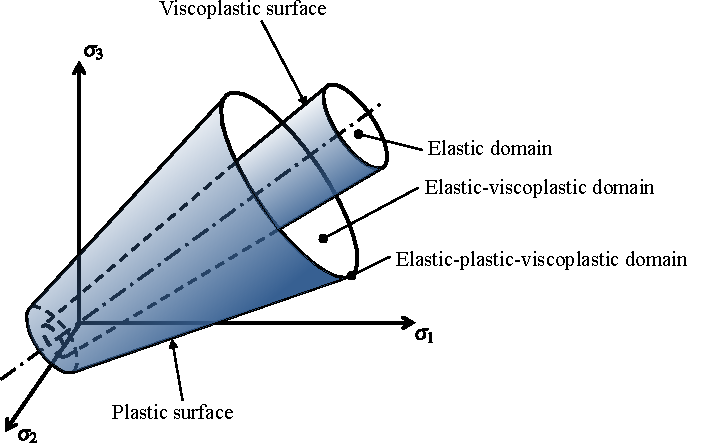
\includegraphics[scale=0.8]{Elastic-plastic-viscoplastic domains.pdf}
	\caption{Elastoplastic-viscoplastic domains.}
	\label{epvpdomains}
\end{figure}

Details of this model, including validations and its application in single tunnel, are in [\citenum{quevedo2022b}]. See [\citenum{quevedo2022thesis}] for the algorithm details implemented in FORTRAN within the USERMAT subroutine.

\section{Constitutive Model of the Lining}\label{}

We implemented a viscoelastic model in ANSYS using the UPF/USERMAT customization feature [\citenum{ANSYS:2013b}]. The model simulates concrete creep through a Generalized Kelvin chain, based on Bažant and Prasannan's Solidification Theory [\citenum{bazant:1989a},  \citenum{bazant:1989b}], with parameter adjustments performed using the CEB-FIP MC90 formulation present in [\citenum{CEB:1993}]. The CEB-FIP MC90 formulation also determines the shrinkage component. 

In this model, the constitutive relationship between stress and strain is 
\begin{equation} \label{eq:8}
	\dstress = \Dll : \dstraine = \Dll : \dstrain - \Dll : \dstrainsh - \Dllmod : \dstraincr\;
\end{equation}
where $\dstrainsh$  and $\dstraincr$ are the shrinkage and creep strain rate, respectively, while $\Dll$ and $\Dllmod$ denote the fourth-order isotropic elastic linear constitutive tensor and modified constitutive tensor that incorporates the aging of the concrete, respectively. Due to the time integration scheme for the Newton-Raphson algorithm, the Eq.~(\ref{eq:8}) is given by:
\begin{equation} \label{eq:9}
	\stress_{n+1} = \stress_{n}+\Dll : \Delta \strain - \Dll : \Delta \strainsh - \Dllmod : \Delta \straincr \;
\end{equation}
in which the increment of shrinkage strain is:
\begin{equation} \label{eq:10}
	\Delta \strainsh =  \Delta \strainshCEB(t_{s}) \onell \;
\end{equation}
where $t_{s}$ represents the concrete curing time, and $\Delta \strainshCEB$ is the variation of magnitude of the concrete deformation by shrinkage, determined using the expressions of CEB-FIP MC90 [\citenum{CEB:1993}]. To calculate the increment of creep strain, denoted as $\Delta \straincr$, we use the incremental algorithm developed by Bažant and Prasannan [\citenum{bazant:1989a,bazant:1989b}], with an adjustment to incorporate CEB-FIP MC90 formulation. This adaptation is possible comparing the creep functions $J(t,t_0)$ of both references. This gives to the following equivalence:
\begin{equation} \label{eq:11}
	E_0 = E_c(t_0),~ \gamma_c(t-t_0)=\beta_c(t-t_0),~ \frac{1}{v(t)} = \frac{\phi_0}{E_{ci}} \text{  and  } \frac{1}{\eta(t)}=0 \;
\end{equation}
in which, according to Bažant and Prasannan [\citenum{bazant:1989a,bazant:1989b}], $E_0$  is the modulus of elasticity of the concrete aggregates and microscopic particles of the cement paste, $\gamma_c(t-t_0)$ is the microviscoelastic deformation of the volume fraction of solidified concrete $v(t)$, $\eta(t)$ is the apparent macroscopic viscosity and, according to CEB-FIP MC90 [\citenum{CEB:1993}], $E_c(t_0)$ is the tangent elastic modulus of the concrete at the instant of loading application $t_0$, $\beta_c(t-t_0)$  is a coefficient that depends on the loading age $t-t_0$ , $\phi_0$ is a coefficient that depends on the age of the concrete at the instant of loading application and $E_{ci}$  the tangent elasticity modulus of the concrete at the age of 28 day.

Details of this model, including validations and its application in single tunnel, are in [\citenum{quevedo2022}]. See [\citenum{quevedo2017comportamento}] for the algorithm details implemented in FORTRAN within the USERMAT subroutine.

\section{Spatial and time discretization of the domain}\label{}

The problem domain $\Omega$ consists of a twin deep tunnel with a cross gallery, as shown in Fig.~\ref{domain}.
\begin{figure}[h!]
	\centering
	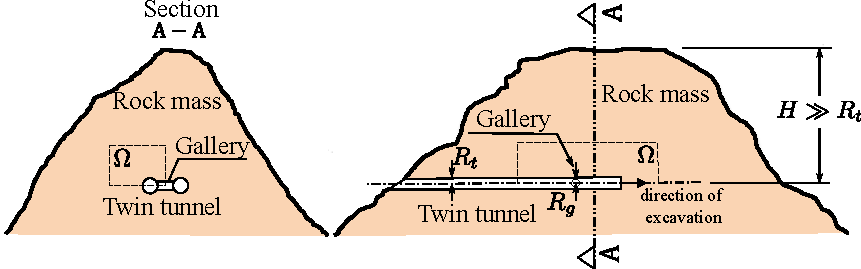
\includegraphics[scale=1]{Domain.pdf}
	\caption{Problem domain}
	\label{domain}
\end{figure}
\FloatBarrier


This domain is parameterized based on the radius of the longitudinal tunnel $R_i$. The geometric parameters and boundary conditions for the domain problem are shown in Fig.~\ref{Mesh1}. We considered front, side, and bottom symmetry to reduce computational cost. In this domain, $d_1$ is the distance between longitudinal tunnel axes, $L_2$ total excavated length, $d_3$ domain height, $L_1$ length of the unexcavated region, $L_3$ transversal length of the domain, $L_p$ step length of the excavation process, $d_2$ position of the gallery along the longitudinal tunnel. In conjunction with boundary pressure $\sigma_x, \sigma_y$ and $\sigma_z$, we apply the initial stress condition $\stress_0 = -\sigma_x \boldsymbol{e}_x \otimes \boldsymbol{e}_x -\sigma_y \boldsymbol{e}_y \otimes \boldsymbol{e}_y -\sigma_z \boldsymbol{e}_z \otimes \boldsymbol{e}_z$ at all integration points to simulate the initial state of the rock mass. The spatial discretization in Fig.~\ref{Mesh1} corresponds to a mesh with trilinear hexahedral elements (SOLID 185, 8 nodes), except in the gallery region, which uses higher-order tetrahedral elements (SOLID186, 10 nodes). 
\begin{figure}[h!]
	\centering
	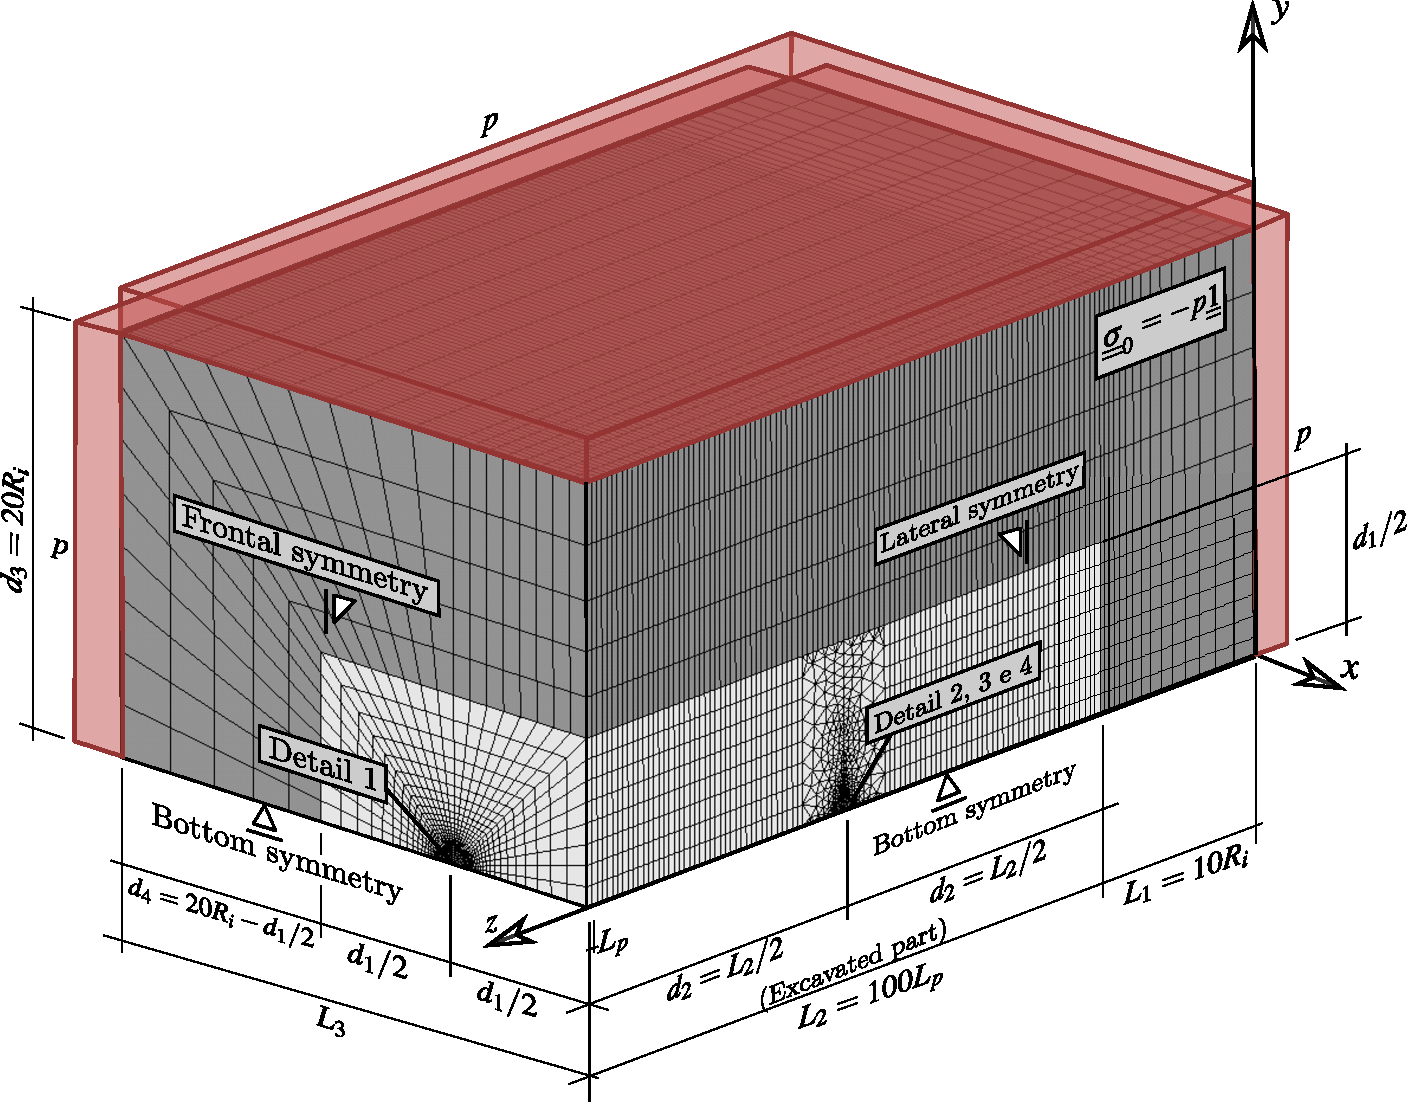
\includegraphics[scale=0.5]{Mesh1.pdf}
	\caption{Mesh, dimensions and boundary conditions of the 3D twin tunnel domain}
	\label{Mesh1}
\end{figure}
We divided the mesh into two regions: one near the tunnel (light gray), which we refined more, and a region farther away (dark gray), which we increased the aspect ratio to minimize the number of elements in that region. Due to the low deformation gradient away from the tunnel wall, elements in this area can be considerably larger than in other regions. Fig.~\ref{Mesh2} presents the mesh at the cross-section of the longitudinal tunnel, with $e$ representing the thickness of the lining.
\begin{figure}[h!]
	\centering
	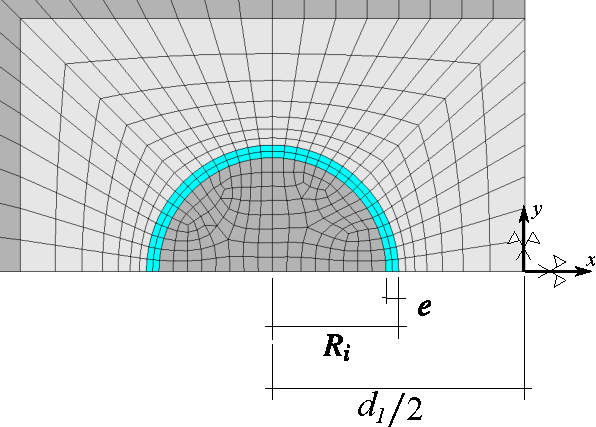
\includegraphics[scale=0.8]{Mesh2.pdf}
	\caption{Detail 1 - Mesh in longitudinal tunnel cross-section with spacing $d_1=4R_i$}
	\label{Mesh2}
\end{figure}
\FloatBarrier
One of the aspects investigated in this work is the influence of the spacing $d_1$ in the convergence of the twin tunnel. Fig.~\ref{Mesh3} and Fig.~\ref{Mesh4} illustrate the spatial discretization in the gallery region and its connection with the longitudinal tunnel considering spacings $d_1 = 16R_i, 8R_i$ and $4R_i$, respectively. We adopt the radius of the gallery as $2/3R_i$, and its lining has the same material and thickness as the longitudinal tunnel. The dimensions $d_5$ and $d_1$ define the size of the transition region comprising tetrahedral elements between the gallery and the rest of the domain. Fig.~\ref{Mesh5} shows half of this transition region inside the rock mass.
\begin{figure}[h!]
	\centering
	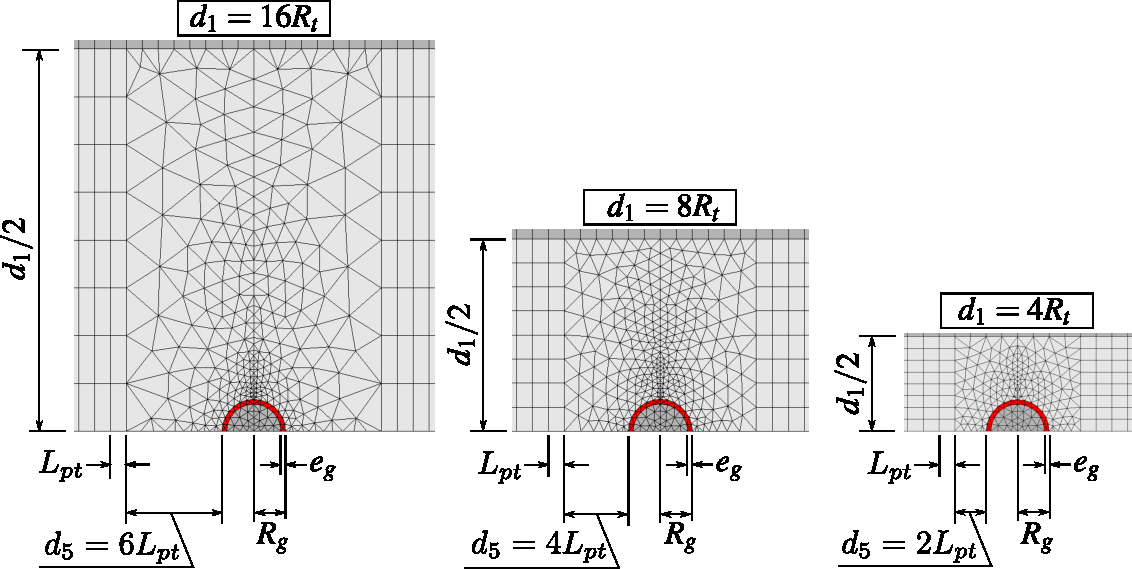
\includegraphics[scale=0.8]{Mesh3.pdf}
	\caption{Detail 2 - Side view of the mesh in gallery region with $d_1=16R_i$, $d_1=8R_i$ and $d_1=4R_i$}
	\label{Mesh3}
\end{figure}
\begin{figure}[h!]
	\centering
	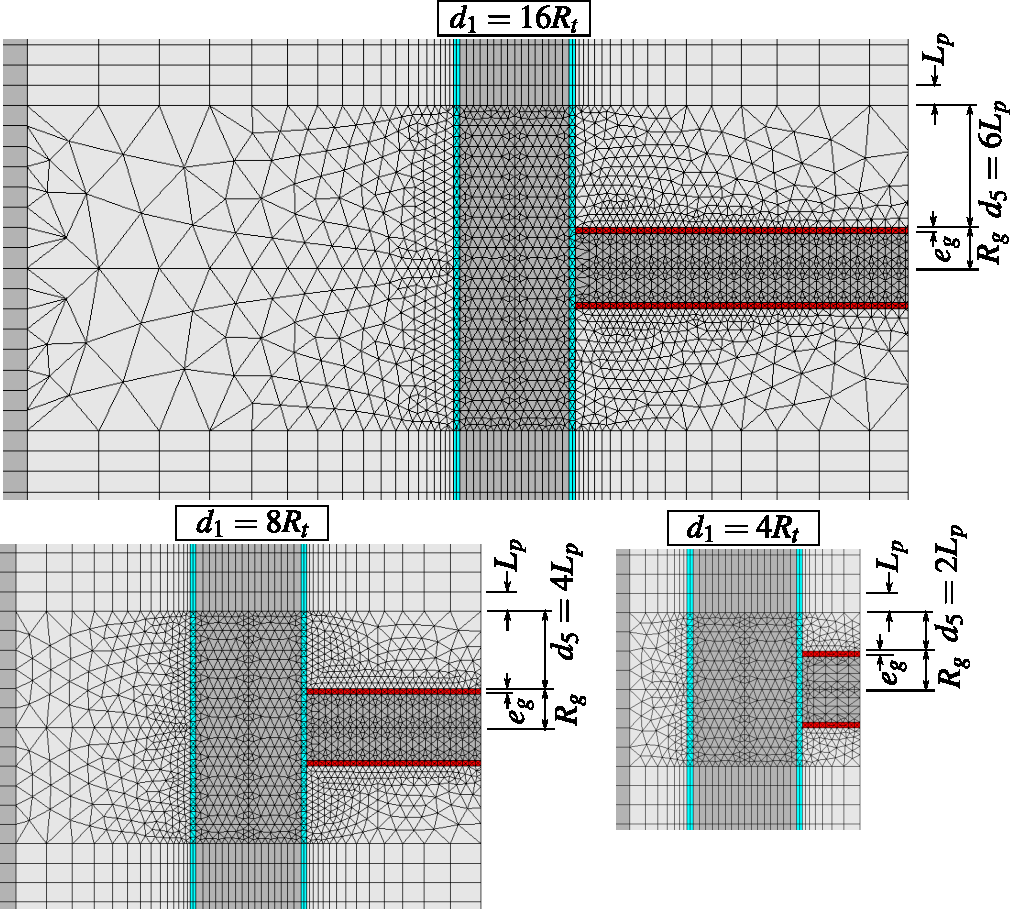
\includegraphics[scale=0.6]{Mesh4.pdf}
	\caption{Detail 3 - Bottom view  of the mesh in gallery region with $d_1=16R_i$, $d_1=8R_i$ and $d_1=4R_i$}
	\label{Mesh4}
\end{figure}
\begin{figure}[h!]
	\centering
	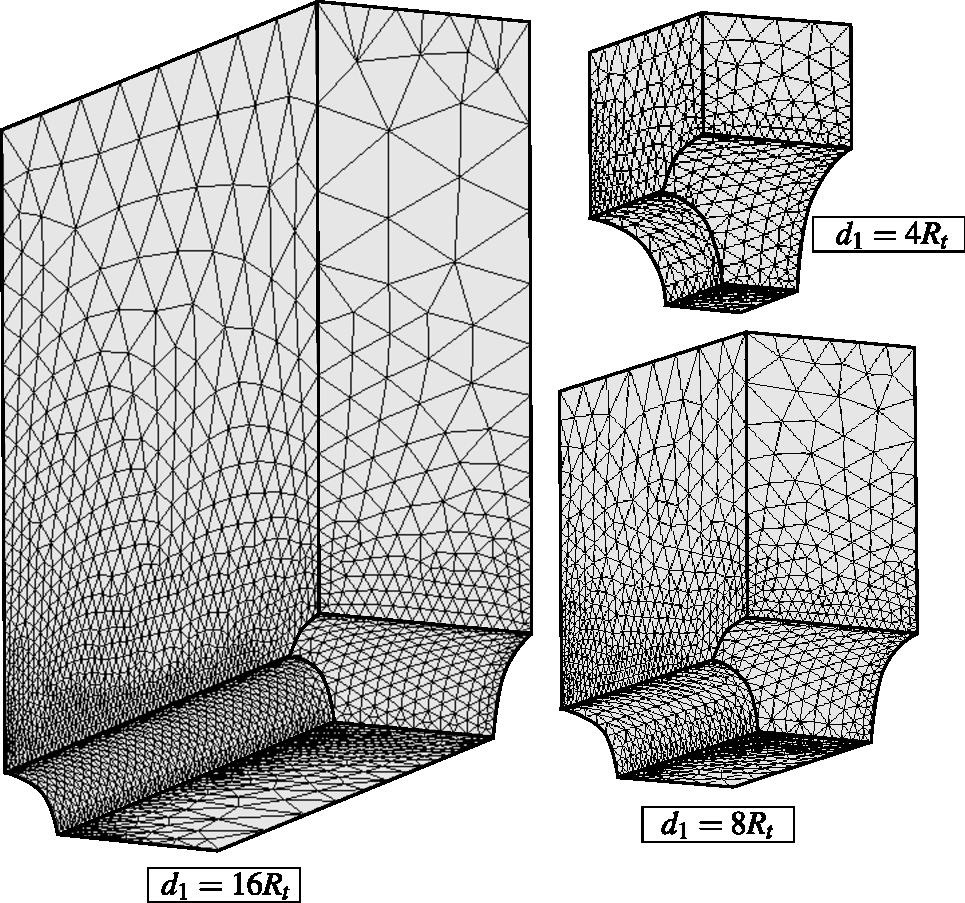
\includegraphics[scale=0.6]{Mesh5.pdf}
	\caption{Detail 4 - Isometric view of the portion of the mesh in gallery transition region $d_1=16R_i$, $d_1=8R_i$ and $d_1=4R_i$}
	\label{Mesh5}
\end{figure}
\FloatBarrier
Fig.~\ref{Mesh6} shows the mesh of the lining at the junction of the gallery and the longitudinal tunnel for $d1 = 4R_i, 8R_i,$ and $16R_i$. One noteworthy characteristic of this mesh is that it confines the tetrahedral elements within the contour of every excavation step.
\begin{figure}[h!]
	\centering
	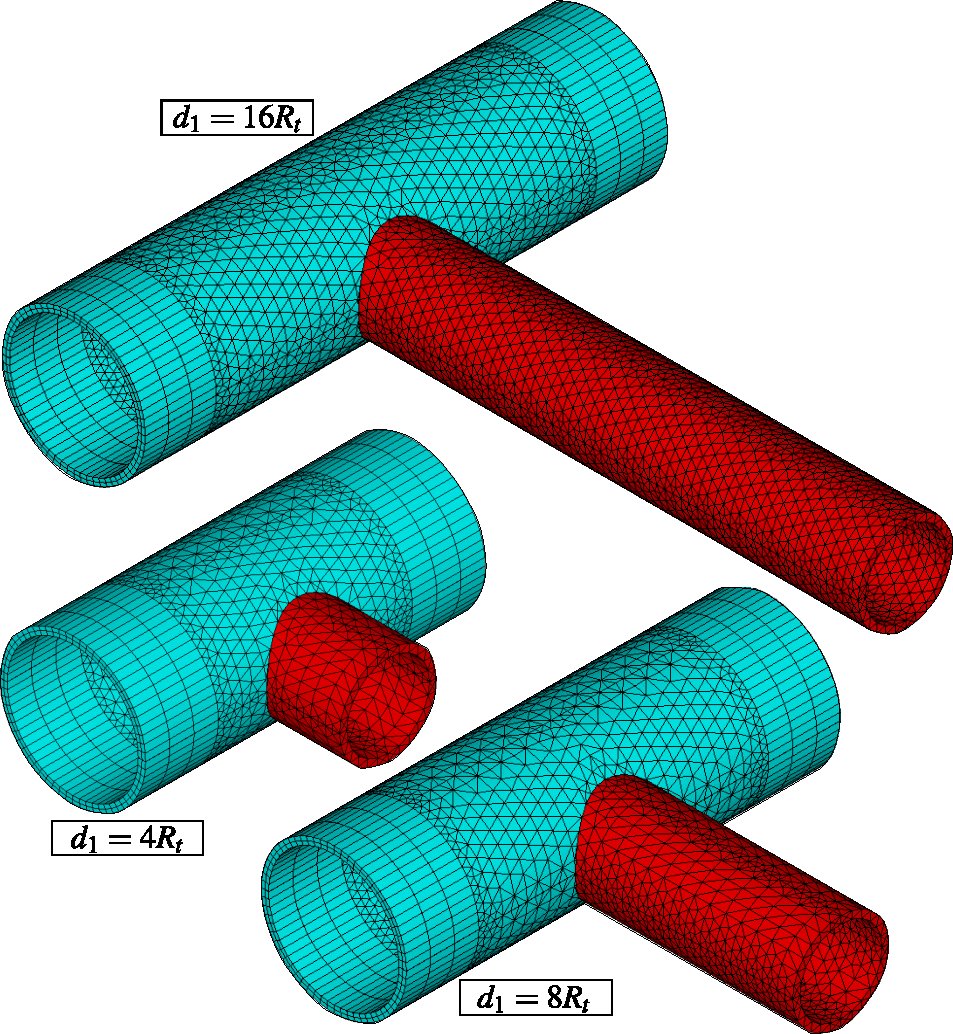
\includegraphics[scale=0.6]{Mesh6.pdf}
	\caption{Isometric view of the lining at the intersection for $d_1=16R_i$, $d_1=8R_i$ and $d_1=4R_i$ - expansion of symmetry in the $xz$ plane}
	\label{Mesh6}
\end{figure}
\FloatBarrier
The construction process is simulated through the deactivating and activating method, i.e., in each step of excavation, reducing the stiffness of the excavated element (multiply  by 1E-8) and active the lining elements at a distance $d_0$ from the excavation face (unlined length). With each excavation step, we execute the solution, and time advances based on the expression $t_p=L_p/V_p$, where $L_p$ represents the length of the excavation step, and $V_p$ is the speed of the excavation face. Fig.~\ref{Diagram of excavations} illustrates a schematic of the excavation process where $n_p$ is the number of excavation steps. In this Figure, $n_{pig}$ represents the number of steps excavated in the longitudinal tunnel that starts gallery excavation. Once reaching this step, we pause the excavation of the longitudinal tunnel, and the gallery excavation begins. In the gallery, $L_{p_1}$ is the step length of the gallery excavation, $V_{p_1}$ is the speed of the gallery excavation, and $d_{0_1}$ is the unlined length of the gallery. After completing the gallery excavation, the longitudinal tunnel excavation resumes. These parameters related to the geometry domain, excavation and installation of the lining are shown in Table~\ref{table1}.
\begin{figure}[h!]
	\centering
	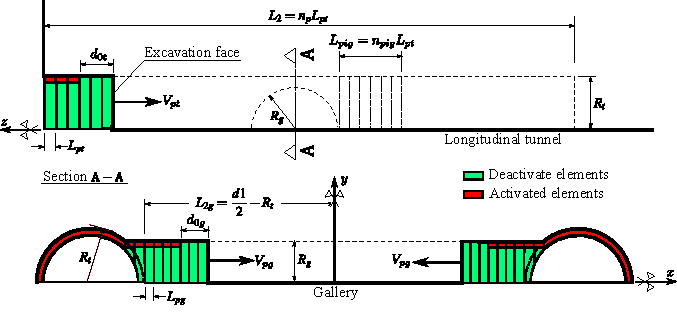
\includegraphics[scale=1.3]{Diagram of excavations.pdf}
	\caption{Schematic of the excavation process}
	\label{Diagram of excavations}
\end{figure}
\FloatBarrier
\begin{table}
	\caption{Parameters related to the geometry of the domain, excavation and installation of the lining}
	\label{table1}
	\centering
	%\small
	\renewcommand{\arraystretch}{1.25}
	\begin{tabular}{c c c c}
		\hline
		\multicolumn{1}{c}{PARAMETERS} &
		\multicolumn{1}{c}{SYMBOL} &
		\multicolumn{1}{c}{UNIT} &
		\multicolumn{1}{c}{VALUES} \\
		\hline
		\multicolumn{4}{c}{Longitudinal tunnels} \\
		\hline
		Radius of the longitudinal tunnel & $R_i$ & m & $R_i$ \\
		Thickness of the lining & $e$ & m & $0.1R_i$ \\
		Step length of the excavation process & $L_p$ & m & $1/3R_i$ \\
		Unlined length & $d_0$ & m & $2L_p$ \\
		Speed of the excavation face & $V_p$ & m/day & 12.5 \\
		Excavation step time & $t_p$ & day & $L_p/V_p$ \\
		\hline
		\multicolumn{4}{c}{Gallery} \\
		\hline
		Radius of the gallery & $R_{i_1}$ & m & $2/3R_i$ \\
		Thickness of the lining & $e_1$ & m & $0.1R_i$ \\
		Step length of the excavation process \footnote{1} & $L_{p_1}$ & m & $0.3R_{i_1} ~0.3214R_{i_1} ~0.3387R_{i_1}$ \\
		Unlined length & $d_{0_1}$ & m & $2L_{p_1}$ \\
		Speed of the excavation face & $V_{p_1}$ & m/day & 12.5 \\
		Number of steps that starts gallery excavation & $n_{pig}$ & un & 15 \\
		\hline
		\multicolumn{4}{c}{Rest of domain} \\
		\hline
		Distance between longitudinal tunnel axes & $d_1$ & m & $4R_i ~8R_i ~16R_i$ \\
		Length of the unexcavated region & $L_1$ & m & $10R_i$ \\
		Total excavated length & $L_2$ & m & $100L_p$ \\
		Domain height & $L_3$ & m & $20R_i$ \\
		\hline
	\end{tabular}
	\normalsize
	\\ \footnotemark[1]{$L_{p_1} \approx 1/3R_{i_1}$ in such a way that there are $n$ integer excavation steps in $d_1-2R_i$}
\end{table}
\FloatBarrier
During tunnel construction, we determine the initial time increment for solution steps as $0.5t_p$ (for the longitudinal tunnel) and $0.5t_{p_1}$ (for the transverse gallery). ANSYS manages the time increment using the bisection method, halving the time step if there is no equilibrium convergence.

After tunnel excavation, in time-dependent constitutive models, time continues to progress to capture long-term viscous effects. In this stage, each time step lasts 100 days, with an initial increment of 50 days. This increase, compared to the excavation time increments, is facilitated by the semi-implicit scheme in the viscoplasticity solution. The explicit scheme, as indicated in [\citenum{zienkiewicz1974visco}], requires a smaller time increment to the precision of the solution.

\section{Comparision with analytical solutions}\label{}

To examine mesh convergence and validate the numerical model, we compared the numerical solution with the elastic and elastoplastic analytical solution in the plane state of deformations for twin tunnels. Guo et al. [\citenum{GUO2021}] develop an elastic analytical solution for the stress field around twin circular tunnels with hydrostatic pressure using the complex variable and the superposition principle. The Fig.~\ref{GUO_FIG1} shows the tangential stress distribution around the tunnel's boundary in this analytical solution with the numerical solution considering  $R_i = 4$ m, $E = 500$ MPa, $\nu =$ 0.23, $d_1 = 2R_i$, $\sigma_x = \sigma_y  = \sigma_z = 2.2$ MPa.
\begin{figure}[h!]
	\centering
	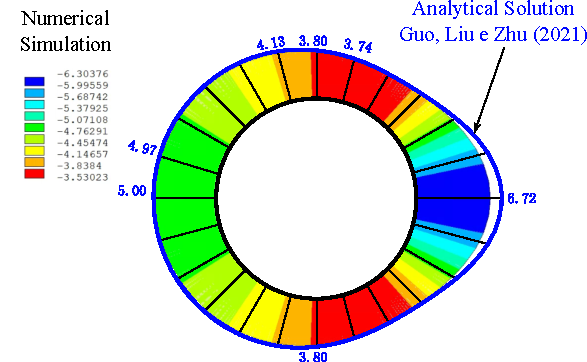
\includegraphics[scale=1]{GUO_FIG1.pdf}
	\caption{Verification of numerical results of orthoradial stresses with the analytical solution}
	\label{GUO_FIG1}
\end{figure}
\FloatBarrier
Ma et. al. [\citenum{MA2020}] developed an analytical solution for a perfectly plastic constitutive model with a Mohr-Coulomb surface. One of the results was the contour of the plastic zone for several conditions. Fig.~\ref{MA_FIG1} shows the comparison between the numerical model solution (taken from a section away from the excavation face) and the analytical solution. For these analysis, $R_i = 1$ m, Young's modulus $E=20$ GPa and Poisson's ratio $\nu = 0.3$.

\begin{figure}[h!]
	\centering
	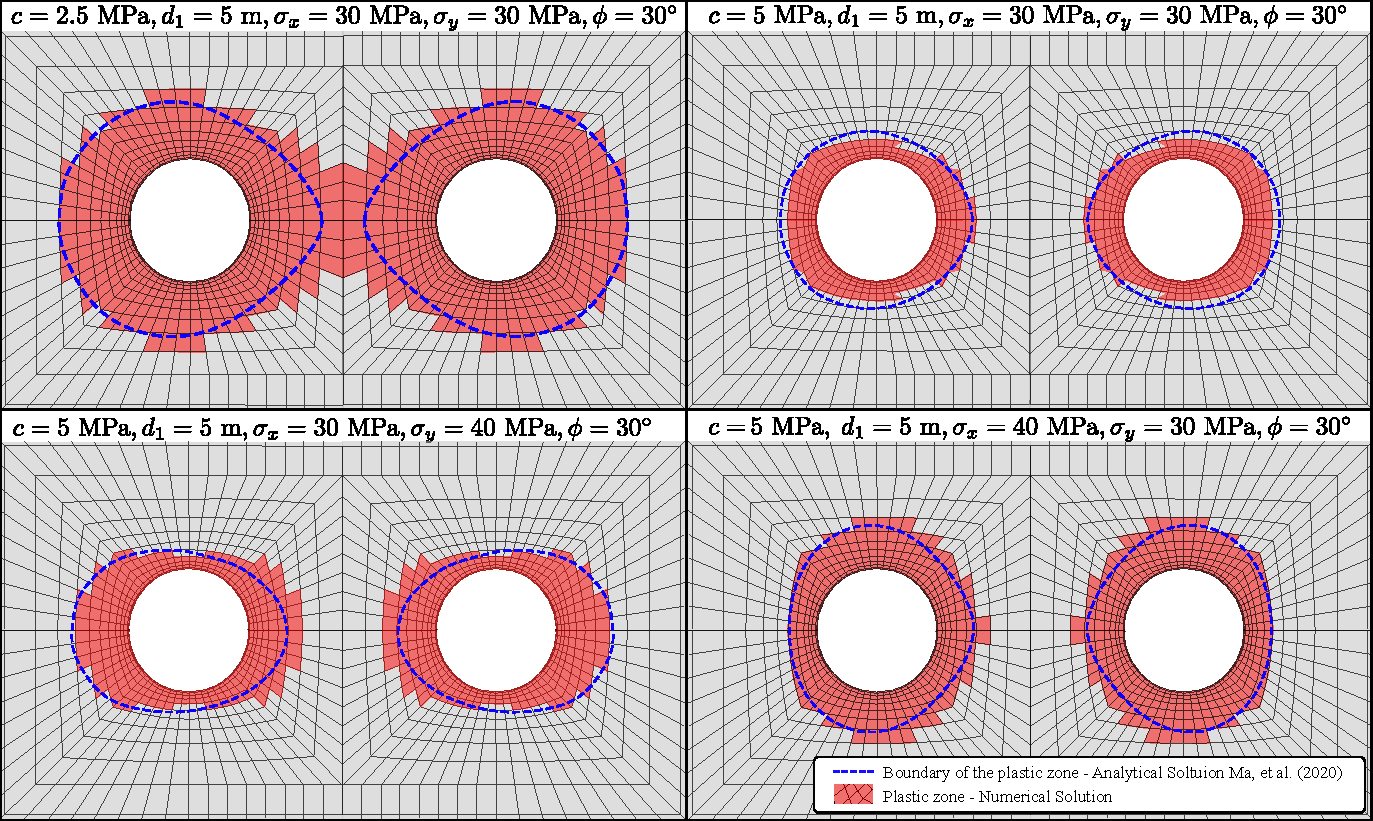
\includegraphics[scale=0.7]{MA_FIG1.pdf}
	\caption{Numerical and analytical comparison of plastic zones}
	\label{MA_FIG1}
\end{figure}
\FloatBarrier

Fig.~\ref{MA_FIG2} displays the magnitude of displacements, radial, orthoradial, and z-direction stresses at the element level  for the case with $c=5$ MPa, $d_1=5$ m, $\sigma_x = \sigma_y = \sigma_z = 30$ MPa. We adopted a case without excavating the gallery to assess the quality of the mesh. The smoothness observed in the solution between the elements indicates satisfactory discretization.

\begin{figure}[h!]
	\centering
	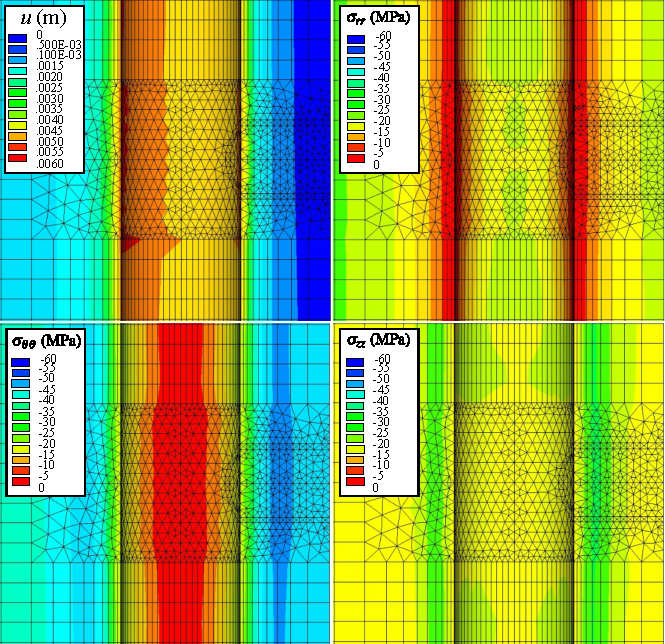
\includegraphics[scale=1]{MA_FIG2.pdf}
	\caption{Element solution with $c=5$ MPa, $d_1=5$ m, $\sigma_x = \sigma_y = 30$ MPa}
	\label{MA_FIG2}
\end{figure}
\FloatBarrier

\section{Numerical Results and Discussion}\label{}

To develop the parametric analyses, we utilized the constitutive parameters of the Callovo-Oxfordian clay rock mass as outlined in Piepi [\citenum{piepi1995}], and for the lining, we employed typical values for ordinary reinforced concrete. These parameters are shown in Table~\ref{table2}. In these analyses the excavation speed is 12.5 m/day.
\begin{table}
	\caption{Constitutive parameters used in the parametric analysis}
	\label{table2}
	\centering
	%\small
	\renewcommand{\arraystretch}{1.25}
	\begin{tabular}{c c c c}
		\hline
		\multicolumn{1}{c}{PARAMETERS} &
		\multicolumn{1}{c}{SYMBOL} &
		\multicolumn{1}{c}{UNIT} &
		\multicolumn{1}{c}{VALUES} \\
		\hline
		\multicolumn{4}{c}{Constitutive model of rock mass} \\
		\hline
		Initial stress state (isotropic) & $\sigma_x, \sigma_y, \sigma_z$ & MPa & 9 \\
		Young's modulus & $E$ & MPa & 1500 \\
		Poisson's ratio & $\nu$ & adm & 0.498 \\
		Plastic cohesion & $c$ & MPa & 4$\sqrt{3}/2$ \\
		Plastic friction angle & $\phi$ & $^{\circ}$ & 0 \\
		Viscoplastic cohesion & $c_{vp}$ & MPa & 2$\sqrt{3}/2$ \\
		Viscoplastic friction angle & $\phi_{vp}$ & $^{\circ}$ & $\phi$ \\
		Power law parameter & $n$ & adm & 1 \\
		Reference parameter & $f_0$ & MPa & 1 \\
		Viscosity coefficient & $\eta$ & day & 40000 \\
		\hline
		\multicolumn{4}{c}{Constitutive model of lining} \\
		\hline
		
		Compressive strength & $f_{ck}$ & MPa & 20 \\
		Young's modulus at 28 days & $E_{c_{28}}$ & MPa & $30303$ \\
		Poisson's ratio & $\nu$ & adm & 0.3 \\
		
		Coefficient which depends on the type of cement & $s$ & adm & 0.2 \\
		Relative humidity of ambient environment & $RH$ & \% & 70 \\
		Fictitious thickness (longitudinal tunnel) & $h_f$ & cm & 0.2111 \\
		Fictitious thickness (transverse gallery) & $h_{f_1}$ & cm & 0.2176 \\
		Drying time of the concrete & $t_s$ & days & 7 \\
		Coefficient in shrinkage which depends on the type of cement & $\beta_{sc}$ & adm & 8 \\
		Temperature & $T$ & $^\circ$C & 20$^\circ$ \\
		Age of concrete at loading & $t_0$ & days & 1 \\
		\hline
	\end{tabular}
	\normalsize
\end{table}
\FloatBarrier
In presenting the results, $U_{eq}$ denotes the equilibrium convergence value at the convergence profile outside the region of influence of the excavation face and the gallery. When the gallery is present, the highest convergence value, $U_{peak}$ is highlighted at the gallery position. In addition, it is necessary to highlight some important points:
\begin{itemize}[]
	\item \textbf{Observation 1}: All the results presented in the following analyses pertain to the point located at the top of the tunnel section (crown), and we will monitor its convergence throughout the excavation process. Fig.~\ref{Ovalization effect and monitoring point} presents this point. Likewise, we will only analyze the convergence of the point located at the crown of the gallery. 
	\item \textbf{Observation 2}: Under material isotropy and initial stress state, the symmetry of the tunnel wall is preserved throughout the excavation process. Thus, the deformed tunnel wall remains circular. On the other hand, one of the effects of the mutual interaction induced by the proximity of the tunnels is the loss of symmetry of the deformed tunnel wall, as illustrated in Fig.~\ref{Ovalization effect and monitoring point}. In this context, the point chosen to follow the convergences (on the crown) is not representative of the entire deformation of the tunnel wall. 
	\item \textbf{Observation 3}: Referring to the material properties shown in Table~\ref{table2}, the value adopted for plastic cohesion ($c$) is higher than the value for viscoplastic cohesion ($c_{vp}$): $c$ > $c_{vp}$. This implies that in the regime of irreversible deformations, the viscoplasticity of the material will be activated first. Throughout the excavation process, viscoplastic deformations will appear without plasticization of the massif. The generic configurations of the deformation zones of the massif throughout the excavation process are illustrated in Fig.~\ref{zones}.
\end{itemize}
\begin{figure}[h!]
	\centering
	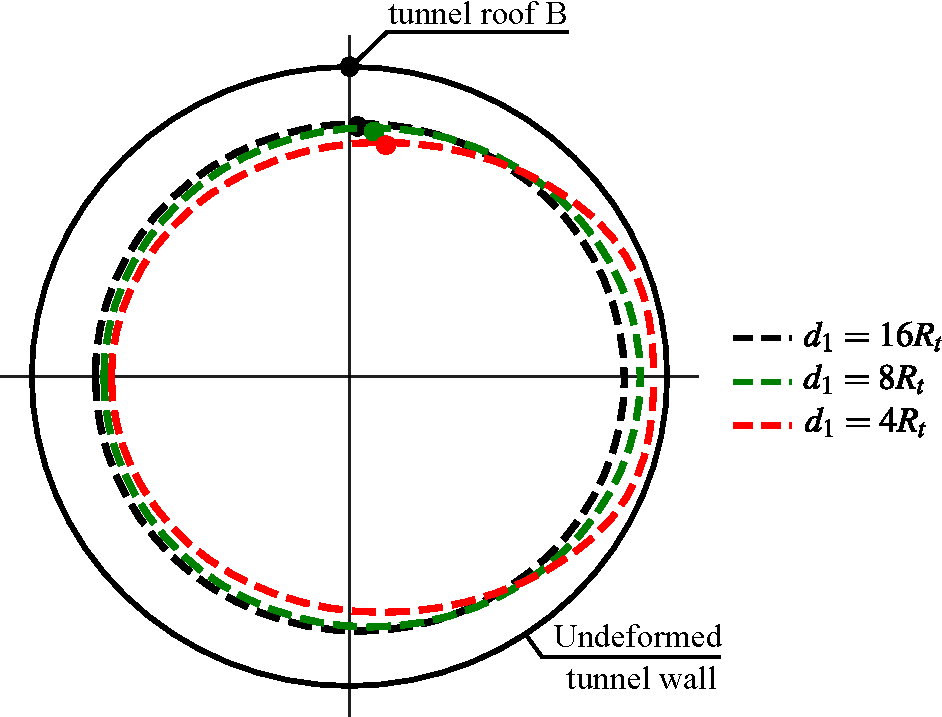
\includegraphics[scale=0.6]{Ovalization effect and monitoring point.pdf}
	\caption{Monitoring point and ovalization effect}
	\label{Ovalization effect and monitoring point}
\end{figure}
\FloatBarrier
\begin{figure}[h!]
	\centering
	\includegraphics[scale=0.6]{zones.pdf}
	\caption{Configurations for the zones with irreversible deformations in the rock mass}
	\label{zones}
\end{figure}
\FloatBarrier
Table~\ref{table3} presents the abbreviation to read the title and legend of the results.
\begin{table}
	\caption{Abbreviation to the title and legend of the results}
	\label{table3}
	\centering
	%\small
	\renewcommand{\arraystretch}{1.25}
	\begin{tabular}{c c}
		\hline
		\multicolumn{1}{c}{DESCRIPTION} &
		\multicolumn{1}{c}{ABBREVIATION} \\
		\hline
		Elastic rock mass & E \\
		Elastoplastic rock mass & EP \\
		Elastoviscoplastic rock mass & VP \\
		Elasto-Plastic-Viscoplastic rock mass & EPVP \\
		Not lining & NL \\
		Elastic lining & EL \\
		Viscoelastic lining & VEL \\
		Long-term & LT \\
		Final excavation (Short-term) & ST \\
		With Gallery & WG \\
		Not Gallery & NG \\			
		\hline
	\end{tabular}
	\normalsize
\end{table}
\FloatBarrier
Figs.~\ref{WG-ST-LT-D1-16RI}, \ref{WG-ST-LT-D1-8RI}, and \ref{WG-ST-LT-D1-4RI} show the convergence profiles of the twin tunnels with gallery (WG) for all the constitutive models of the rock mass (E - blue, EP - yellow, VP - magenta, EPVP - red) and the lining (EL and VEL) in the short-term (solid lines) and the long-term (dashed lines), for $d_1 = 16R_i, 8Ri$ and $4R_i$ respectively.
\begin{figure}[h!]
	\centering
	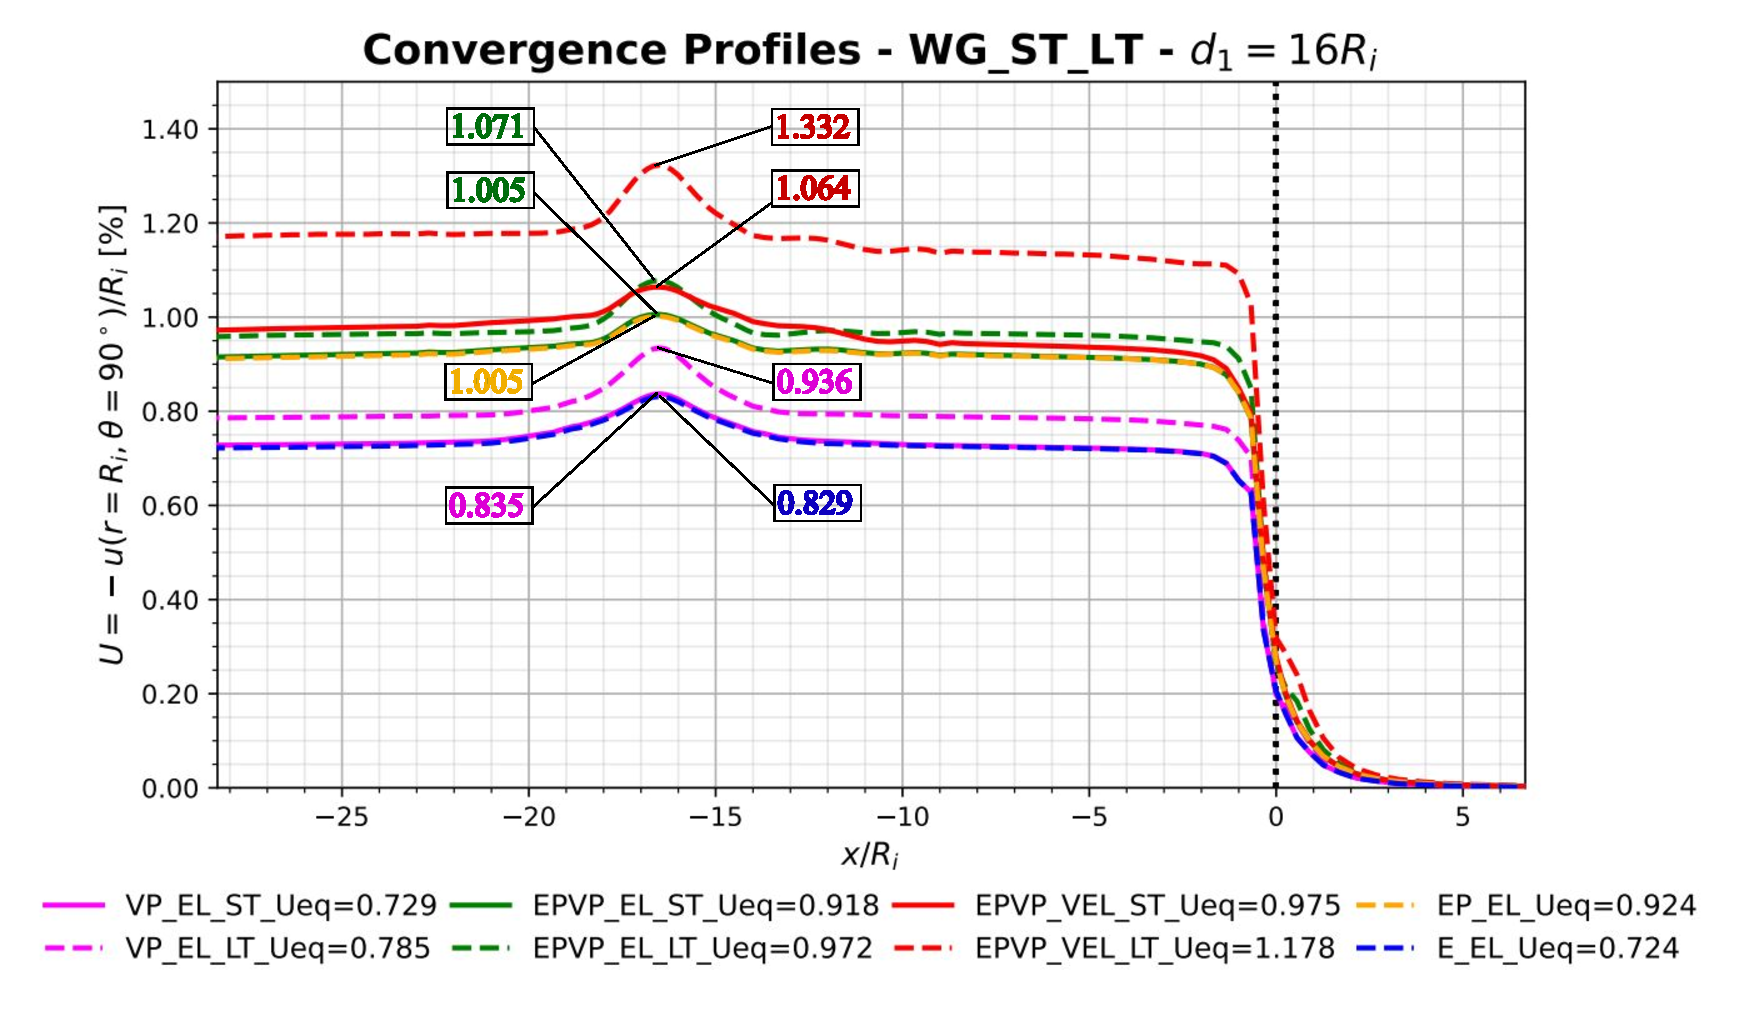
\includegraphics[scale=0.5]{Convergence Profiles - WG_ST_LT - $d_1=16R_i$.pdf}
	\caption{Convergence Profiles - with gallery (WG), short-term (ST) and long-term (LT) for $d_1 = 16R_i$}
	\label{WG-ST-LT-D1-16RI}
\end{figure}
\FloatBarrier
\begin{figure}[h!]
	\centering
	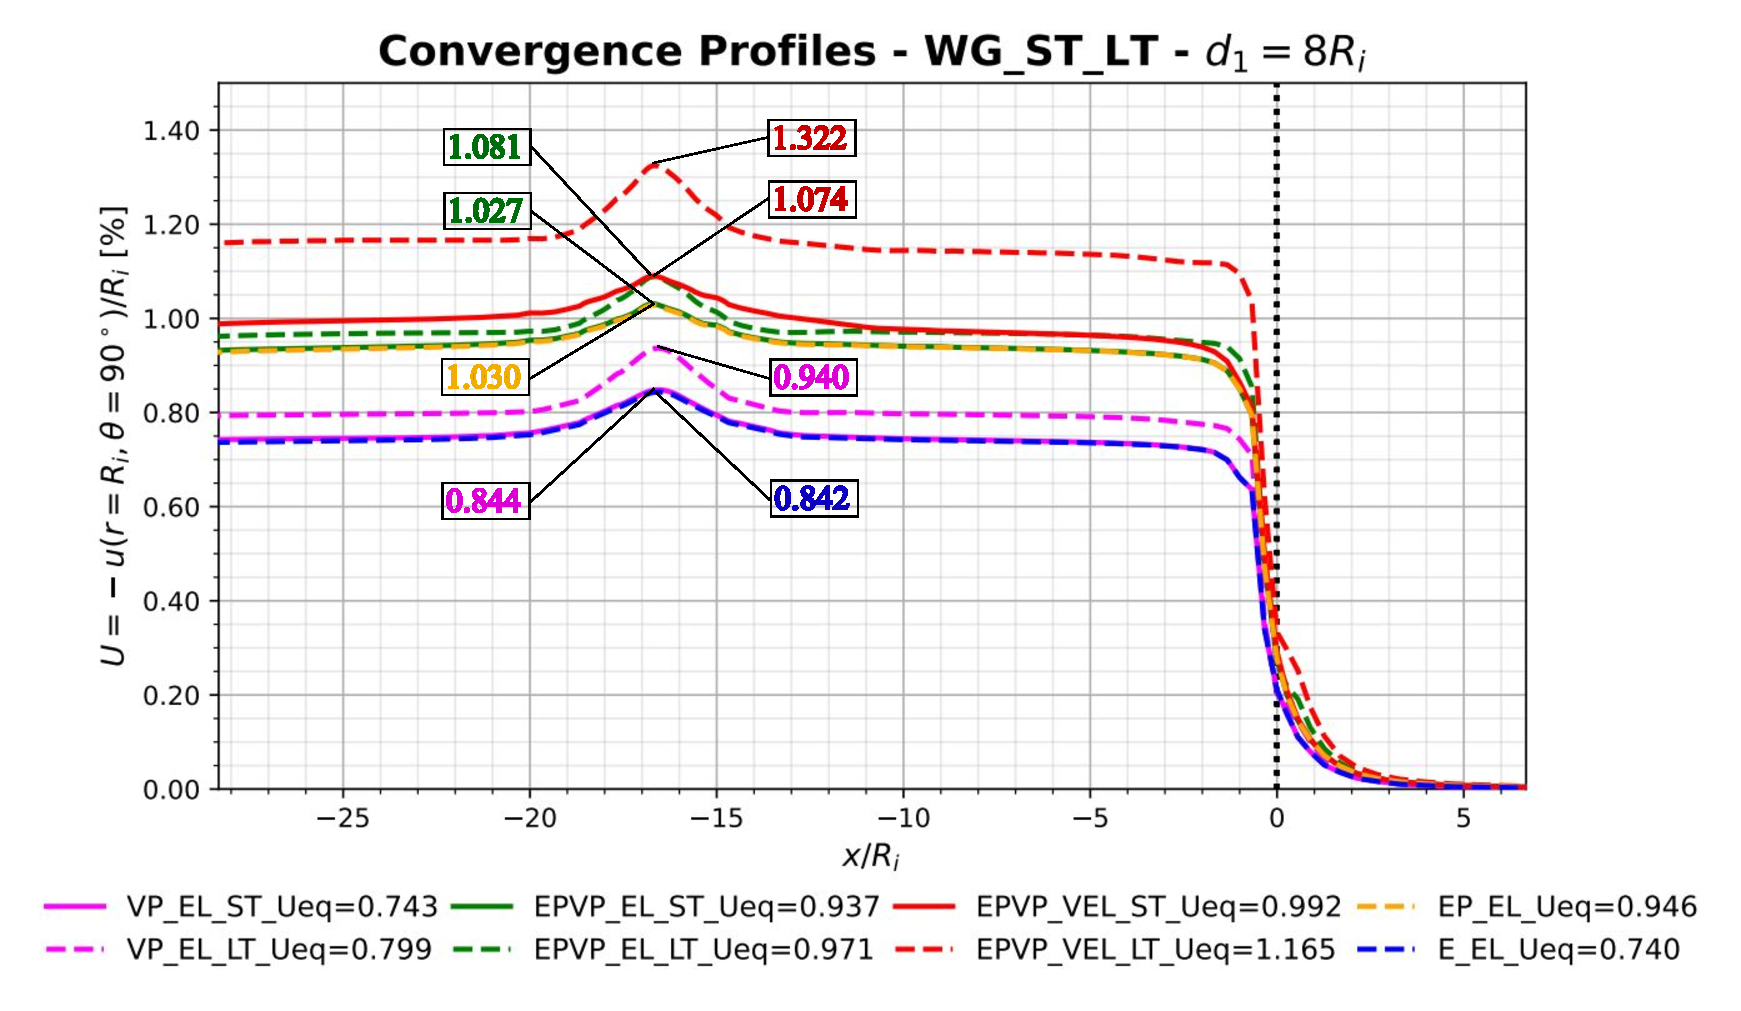
\includegraphics[scale=0.5]{Convergence Profiles - WG_ST_LT - $d_1=8R_i$.pdf}
	\caption{Convergence Profiles - with gallery (WG), short-term (ST) and long-term (LT) for $d_1 = 8R_i$}
	\label{WG-ST-LT-D1-8RI}
\end{figure}
\FloatBarrier
\begin{figure}[h!]
	\centering
	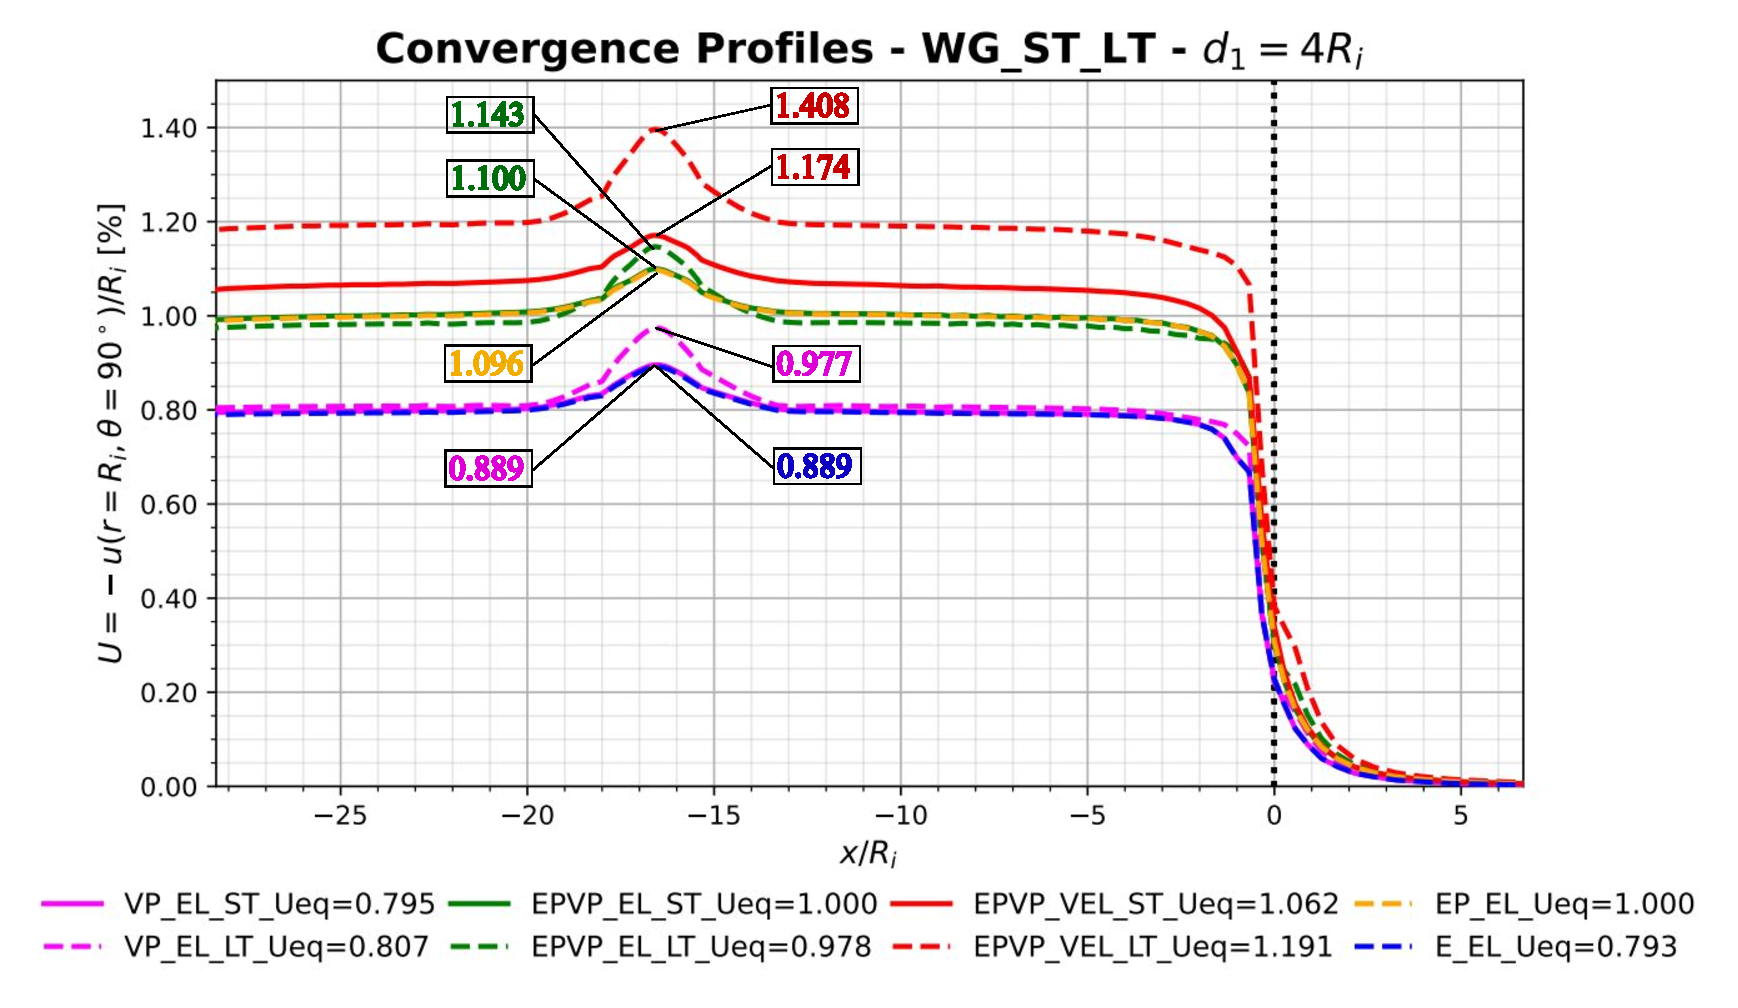
\includegraphics[scale=0.5]{Convergence Profiles - WG_ST_LT - $d_1=4R_i$.pdf}
	\caption{Convergence Profiles - with gallery (WG), short-term (ST) and long-term (LT) for $d_1 = 4R_i$}
	\label{WG-ST-LT-D1-4RI}
\end{figure}
\FloatBarrier
In all $d_1$ distances, the convergence profiles of the E-EL model (blue dashed line) and the VP-EL (magenta solid line) in the short-term (ST) are equivalent, probably due to the high excavation speed. The high speed of the excavation and installation of the lining limits the time for the viscous effects to manifest themselves also taking into account the restriction imposed by the stiffness of the lining.

In the short-term (ST), the EPVP-EL model (green solid line) is equivalent to the EP-EL (yellow dashed line) because, although plasticization around the section has already occurred due to excavation, the viscous effects have not yet evolved considerably due to the short time variation between the start of excavation and the end of the excavation process. After the long-term convergence occurs (green dashed line) are a difference. However, when the rheological effect of the lining is present, the profile continues to evolve considerably over the long-term, for example, EPVP-VEL (red solid and dashed line).

It's worth noting that the stiffness of the elastic lining significantly impedes the evolution of convergence due to viscous effects, particularly evident in the VP-EL model with $d_1=4R_i$ (magenta solid and dashed line). In this scenario, the interaction between nearby twin tunnels causes a substantial rise in the value of $U_{eq}$ in the short-term (ST). However, the profile in the long-term (LT) practically remains unchanged, staying close to the short-term due to the limitation imposed by the stiffness of the lining.

Another noteworthy aspect is that the EPVP-VEL model with $d_1 = 16R_i$ (red dashed line) experiences a reduction in $U_{eq}$ convergence after 15 excavation steps ($n_{pig}$) following the gallery. This phenomenon is due to the evolving viscous effects of the already-excavated longitudinal tunnel during the gallery excavation. This effect becomes more pronounced with $d_1 = 16R_i$. When the gallery is smaller ($d_1 = 8R_i$ and $4R_i$), the time elapsed is shorter, and this effect is less pronounced.

Note another aspect: the EPVP-EL-LT (green solid line) model converges slightly lower than the EVP-EL-ST (green dashed line) model with $d_1 = 4R_i$. The ovalization effect is responsible for the crown's convergence decreasing over time. However, another point in the section experiences an increase in convergence. Fig.~\ref{ovalization} illustrates this effect away from the gallery region with a single tunnel reference.
\begin{figure}[h!]
	\centering
	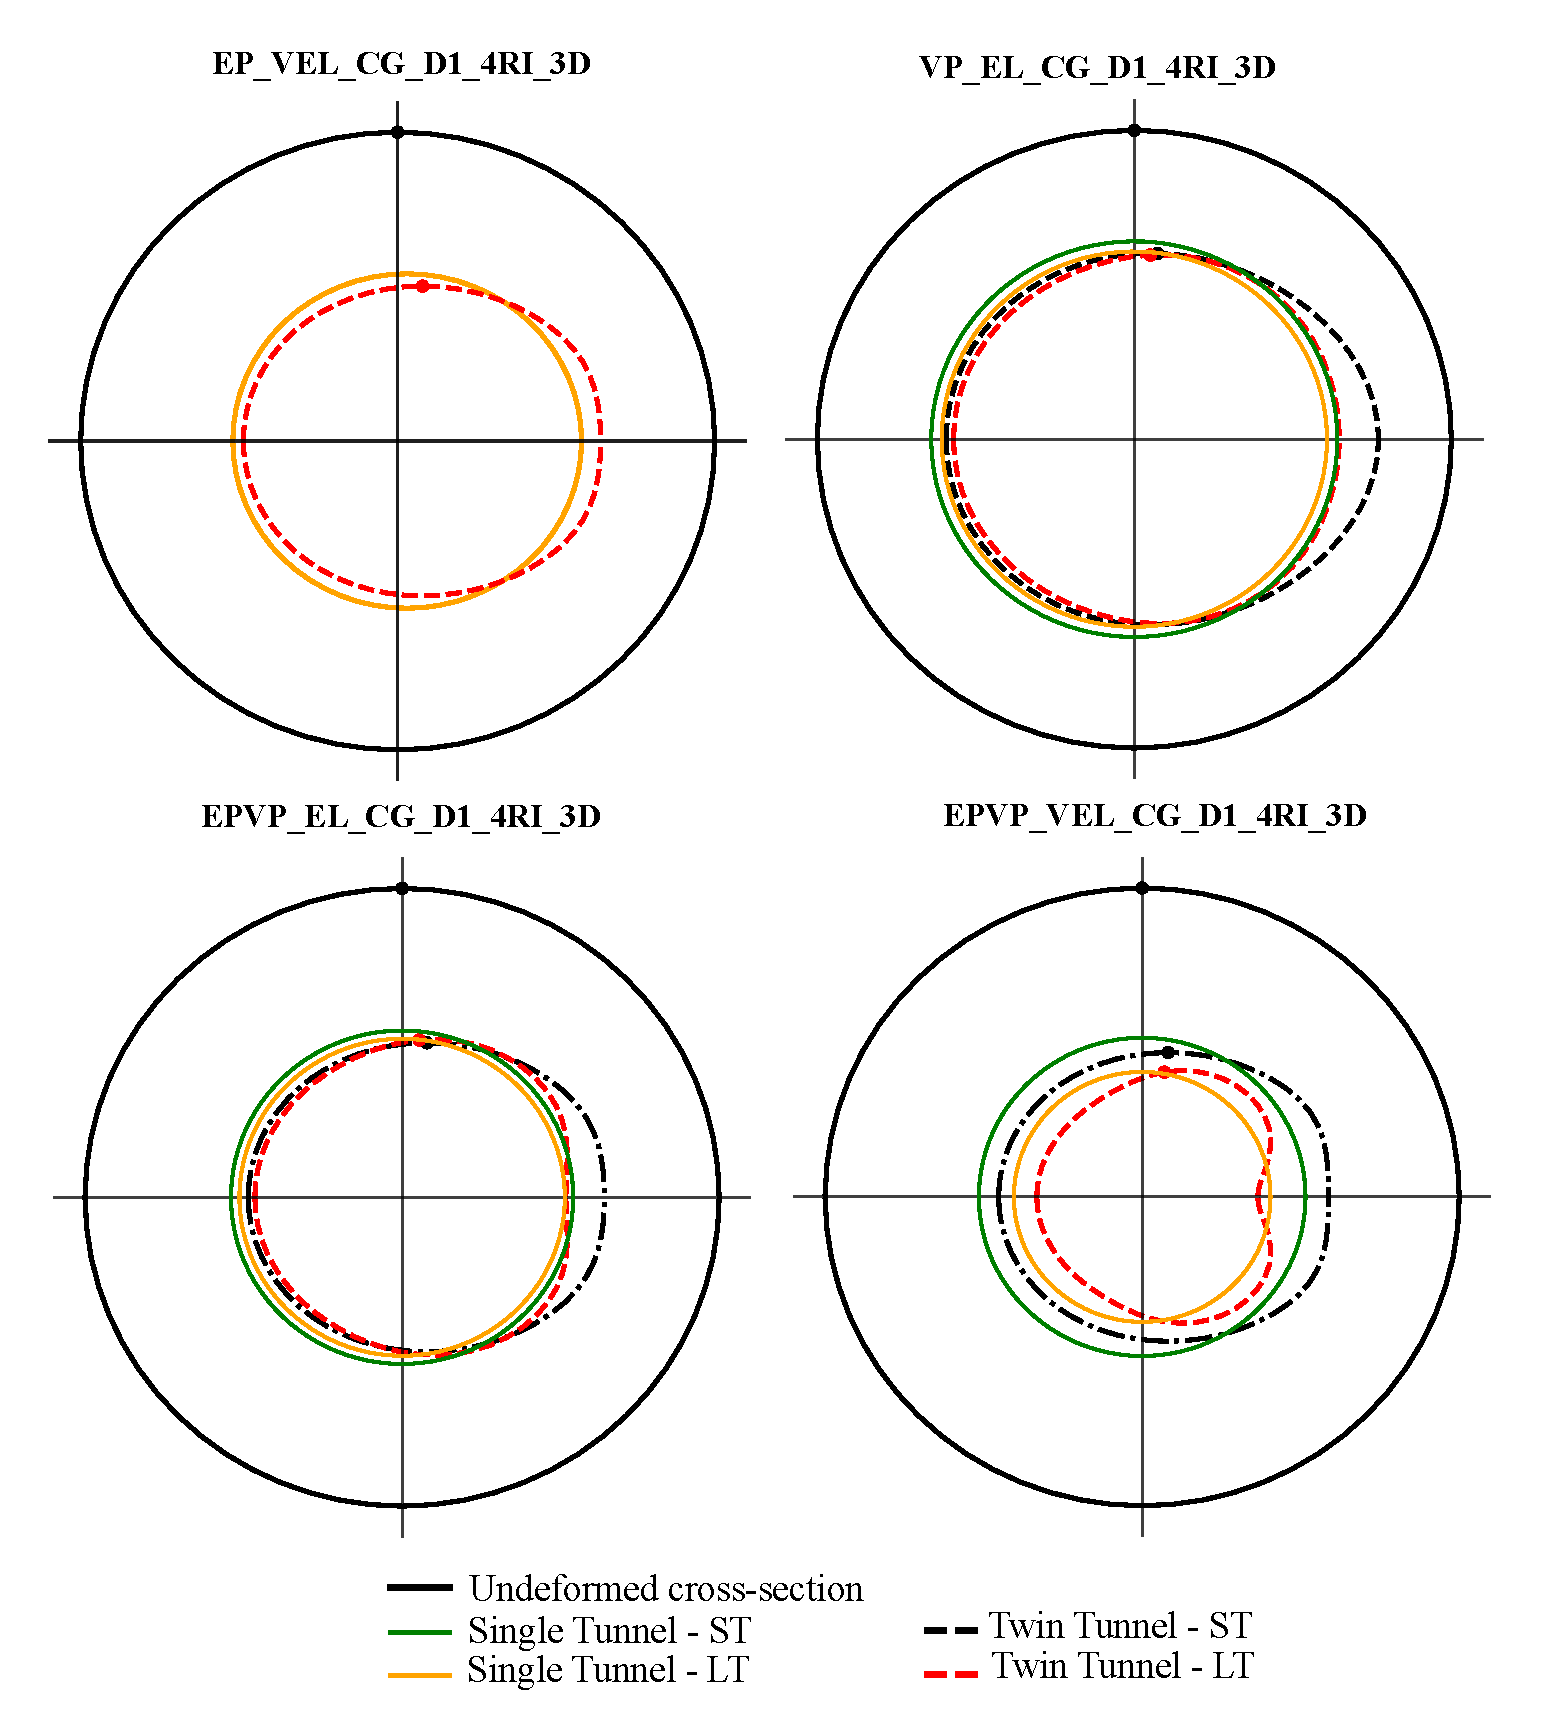
\includegraphics[scale=0.5]{ovalization.pdf}
	\caption{Ovalization effect for $d_1 = 4R_i$ scaled 50x}
	\label{ovalization}
\end{figure}
\FloatBarrier
Fig.~\ref{VP-EL-EPVP-VEL-WG-LT} compares the convergence profiles of the viscoplastic rock mass (VP) with elastic lining (EL) models (solid lines) with the elasto-plastic-viscoplastic rock mass (EPVP) with elastic (EL) and viscoelastic lining (VEL) models in the long-term (LT) (dashed lines and dot lines, respectively). As a reference, it also shows the results for a single tunnel (black lines).
\begin{figure}[h!]
	\centering
	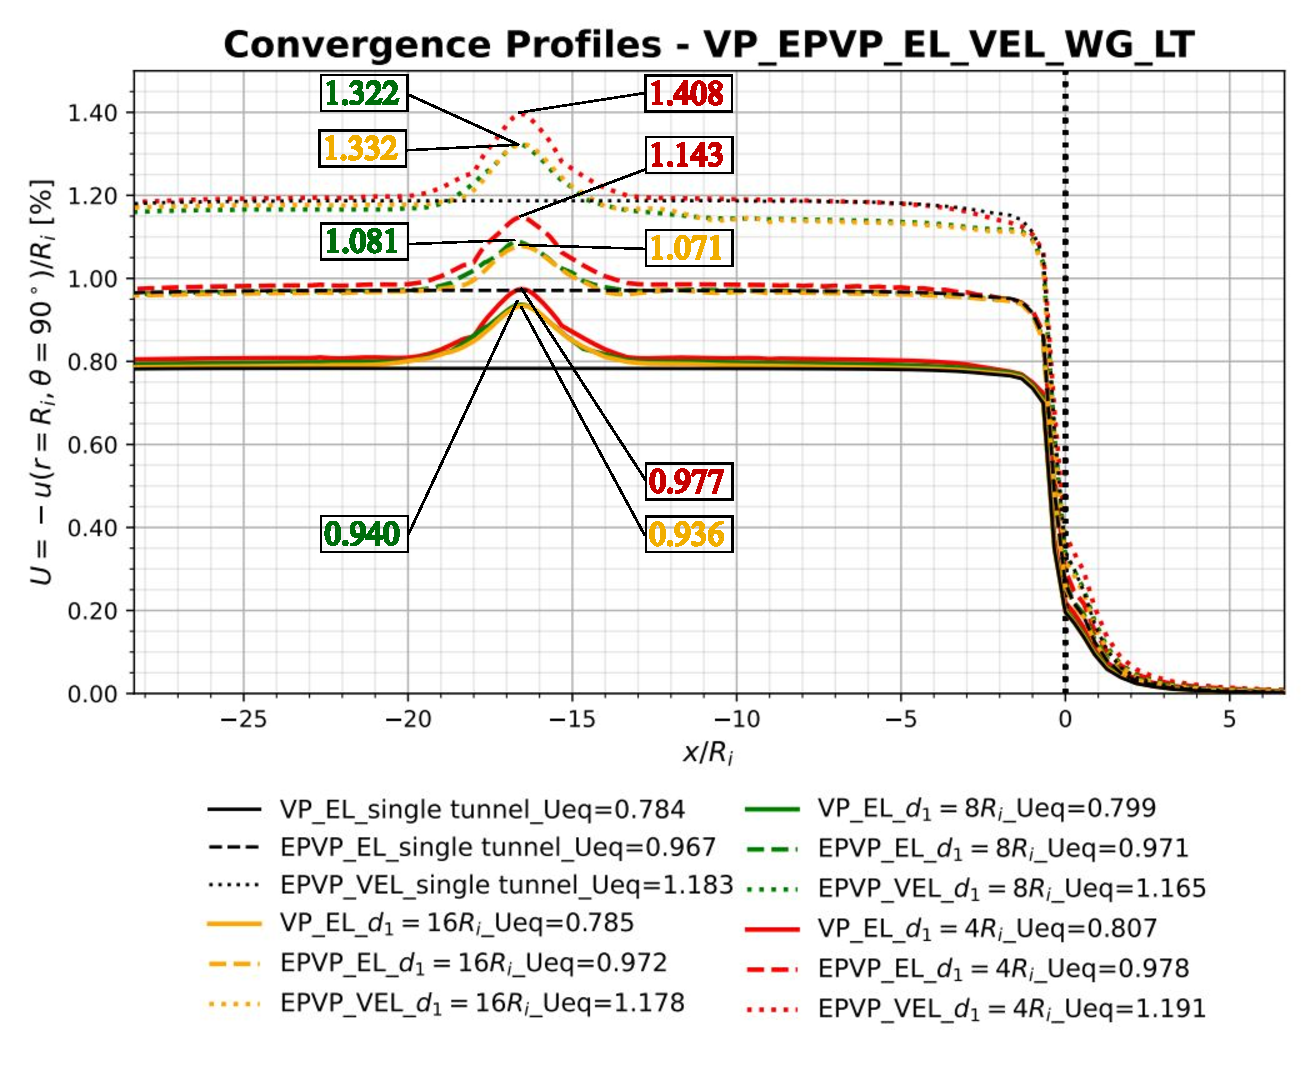
\includegraphics[scale=0.6]{Convergence Profiles - VP_EPVP_EL_VEL_WG_LT.pdf}
	\caption{Convergence Profiles - viscoplastic rock mass (VP) with elastic lining (EL) versus elasto-plastic-viscoplastic rock mass (EPVP) with elastic (EL) and viscoelastic lining (VEL) in long-term (LT)}
	\label{VP-EL-EPVP-VEL-WG-LT}
\end{figure}
\FloatBarrier
Figure \ref{VP-EL-EPVP-VEL-WG-LT} shows a slight increase in the peak value of convergence $U_{peak}$ for the EPVP-VEL model when comparing $d_1 = 16R_i$ (dotted yellow line) and $d_1 = 8R_i$ (dotted green line). In the case of $d_1 = 8R_i$, the proximity of the tunnel compensates the convergence difference due the gallery excavation eplapsed time between $d_1 = 8R_i$ and $16 R_i$. However, when $d_1 = 4R_i$ (dotted red line) the effect of the gallery is more pronounced due to the interaction between the proximity of the twin tunnels and the viscous effect. 

Moreover, one can observe a more pronounced effect in the section before the gallery, specifically at the plateau of the convergence profile, in the EPVP-VEL model for $d_1 = 8R_i$ and $d_1 = 16R_i$ (green and yellow dotted lines). This effect is due to the viscoelastic behavior of the lining and elapsed time to excavate the gallery. Unlike the highly rigid elastic lining, the viscoelastic lining allows the convergence to evolve during the excavation of the gallery. Consequently, the values of convergences before the gallery tend to be higher than after the gallery.

Fig.~\ref{EP-EL-EPVP-VEL-WG-ST-LT} compares the convergence profiles of the elastoplastic rock mass (EP) and elastic lining (EL) models (solid lines) with the elasto-plastic-viscoplastic rock mass (EPVP) and viscoelastic lining (VEL) models in the short-term (ST) (dot lines) and long-term (LT) (dahed lines). As a reference, it also shows the results for a single tunnel (black lines).
\begin{figure}[h!]
	\centering
	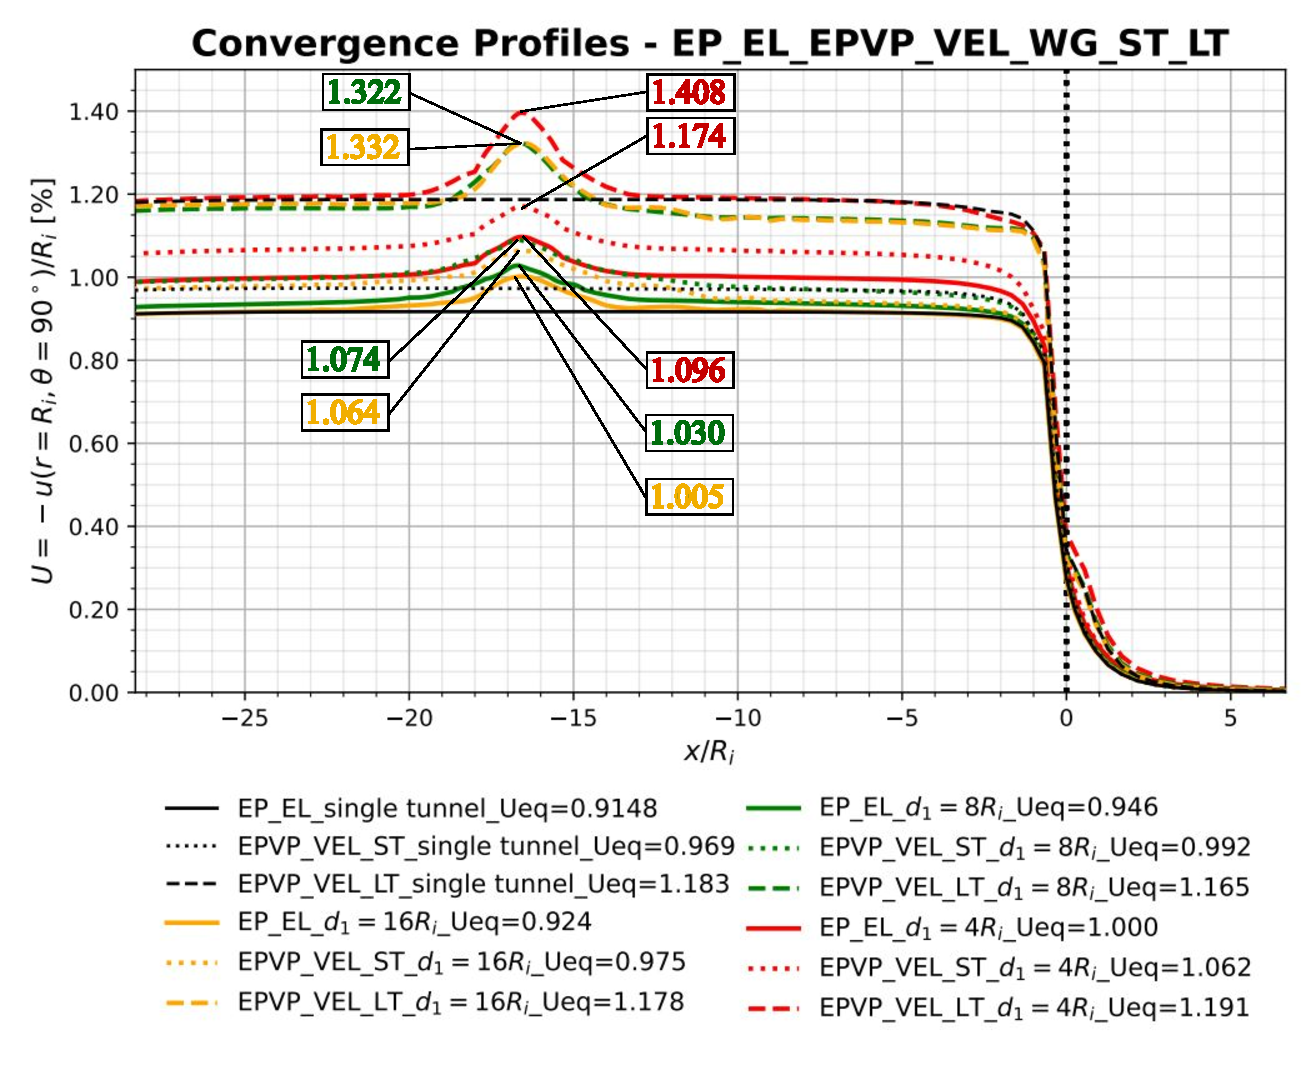
\includegraphics[scale=0.6]{Convergence Profiles - EP_EL_EPVP_VEL_WG_ST_LT.pdf}
	\caption{Convergence Profiles - elastoplastic rock mass (EP) with elastic lining (EL) versus elasto-plastic-viscoplastic rock mass (EPVP) with viscoelastic lining (VEL) in short-term (ST) and long-term (LT)}
	\label{EP-EL-EPVP-VEL-WG-ST-LT}
\end{figure}
\FloatBarrier
This Figure shows the crucial effect of the viscoelastic lining to the convergence profile of the tunnels. In the short term (ST), the elastoplastic-viscoplastic rock mass (EPVP) with viscoelastic lining (VEL) (dotted lines) shows superior convergences compared to the elastoplastic (EP) model with elastic lining (EL) (solid lines). Because the young age of the viscoelastic lining (VEL) has a lower modulus of elasticity, resulting in lower stiffness. Therefore, compared to the elastic lining (EL), the lower initial value of the modulus of elasticity contributes more to the development of convergence. In the long term (LT), even though the viscoelastic lining (VEL) (dashed lindes) has a higher stiffness due to a aging of lining, the viscous effects over time result in a significantly more discrepant convergence profile compared to the elastoplastic model (EP) with elastic lining (EL) (solid lines). There is a noticeable increase in the magnitude of $U_{peak}$ between the short term and the long term at the gallery position, highlighting the influence of the viscoelastic lining.

To study the effect of the lining, Fig.~\ref{EP_d1_16Ri} and \ref{EP_d1_4Ri} show the elastoplastic rock mass (EP) under various conditions: without lining (NL), with a moderately stiff elastic lining ($K_c = 1027$ MPa), and with a highly stiff lining ($K_c = 3660$ MPa) with (WG) and without gallary (NG).
\begin{figure}[h!]
	\centering
	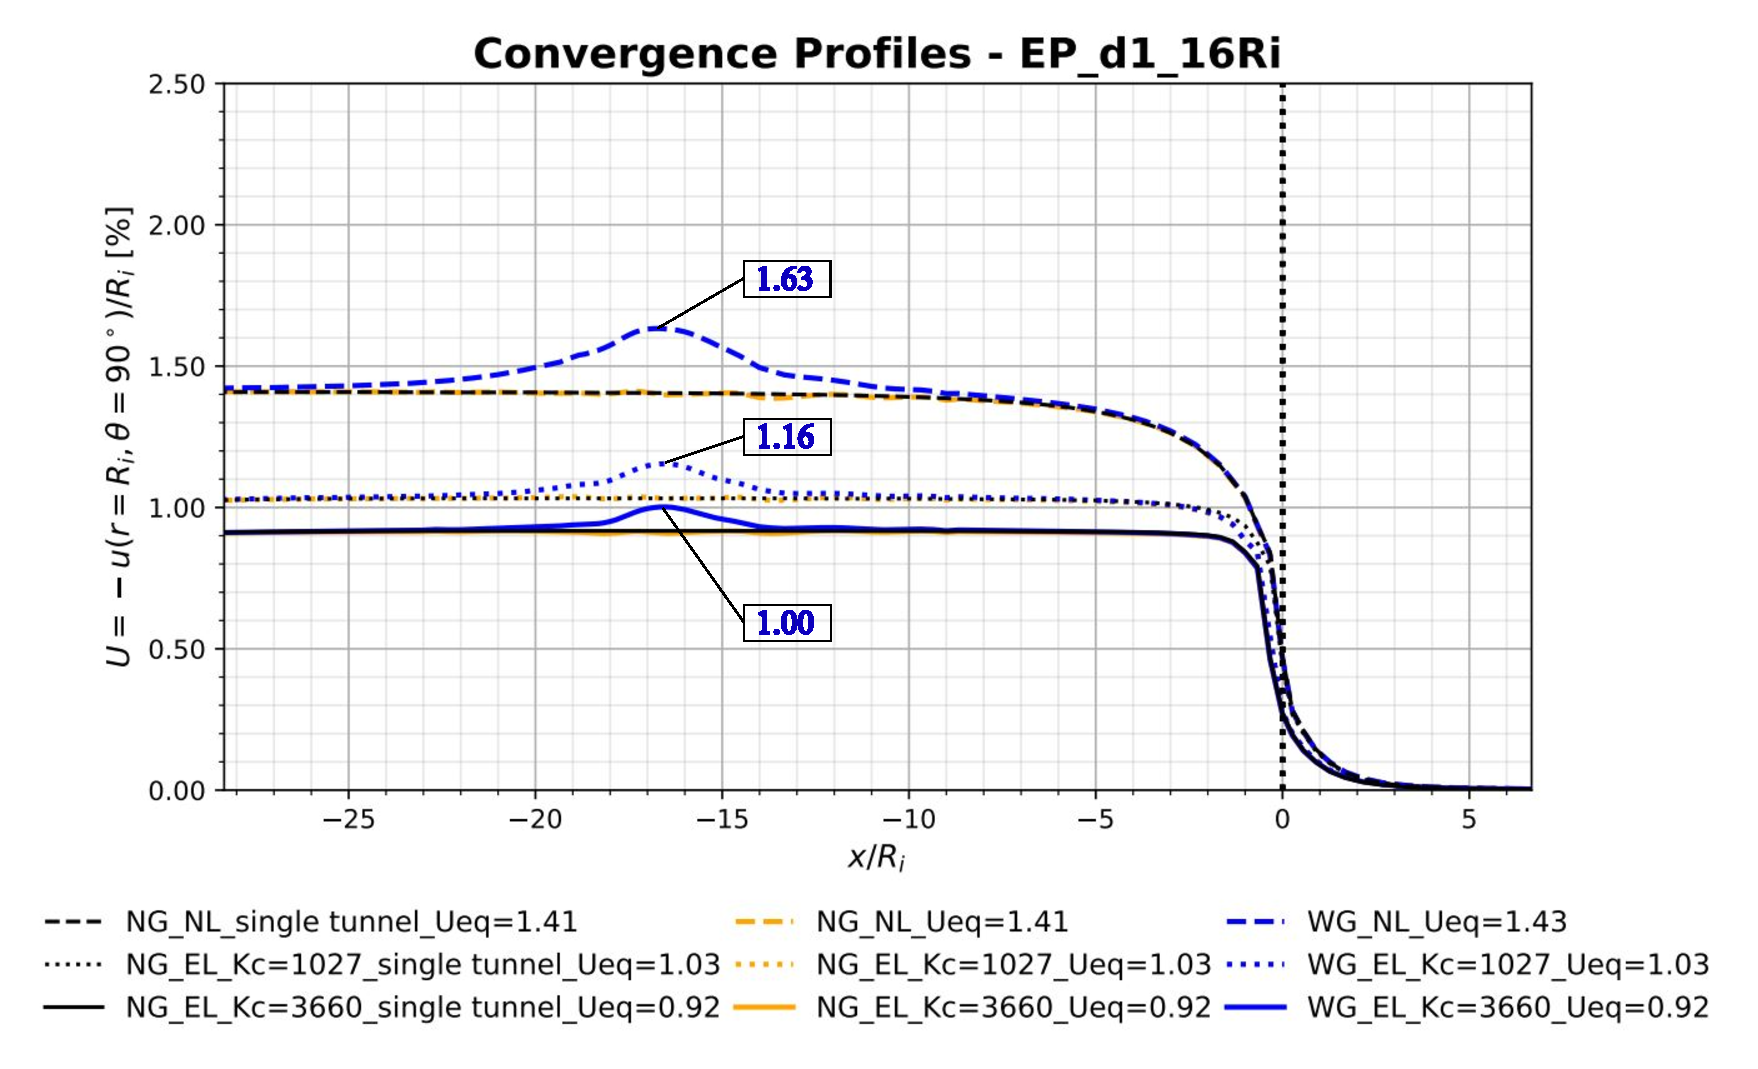
\includegraphics[scale=0.5]{Convergence Profiles - EP_d1_16Ri.pdf}
	\caption{Convergence Profiles - elastoplastic rock mass (EP) without lining (NL) with a highly stiff elastic lining ($K_c = 3660$ MPa) and a moderately stiff elastic lining ($K_c = 1027$ MPa), without (NG) and with gallery (WG) for $d_1 = 16R_i$}
	\label{EP_d1_16Ri}
\end{figure}
\FloatBarrier
\begin{figure}[h!]
	\centering
	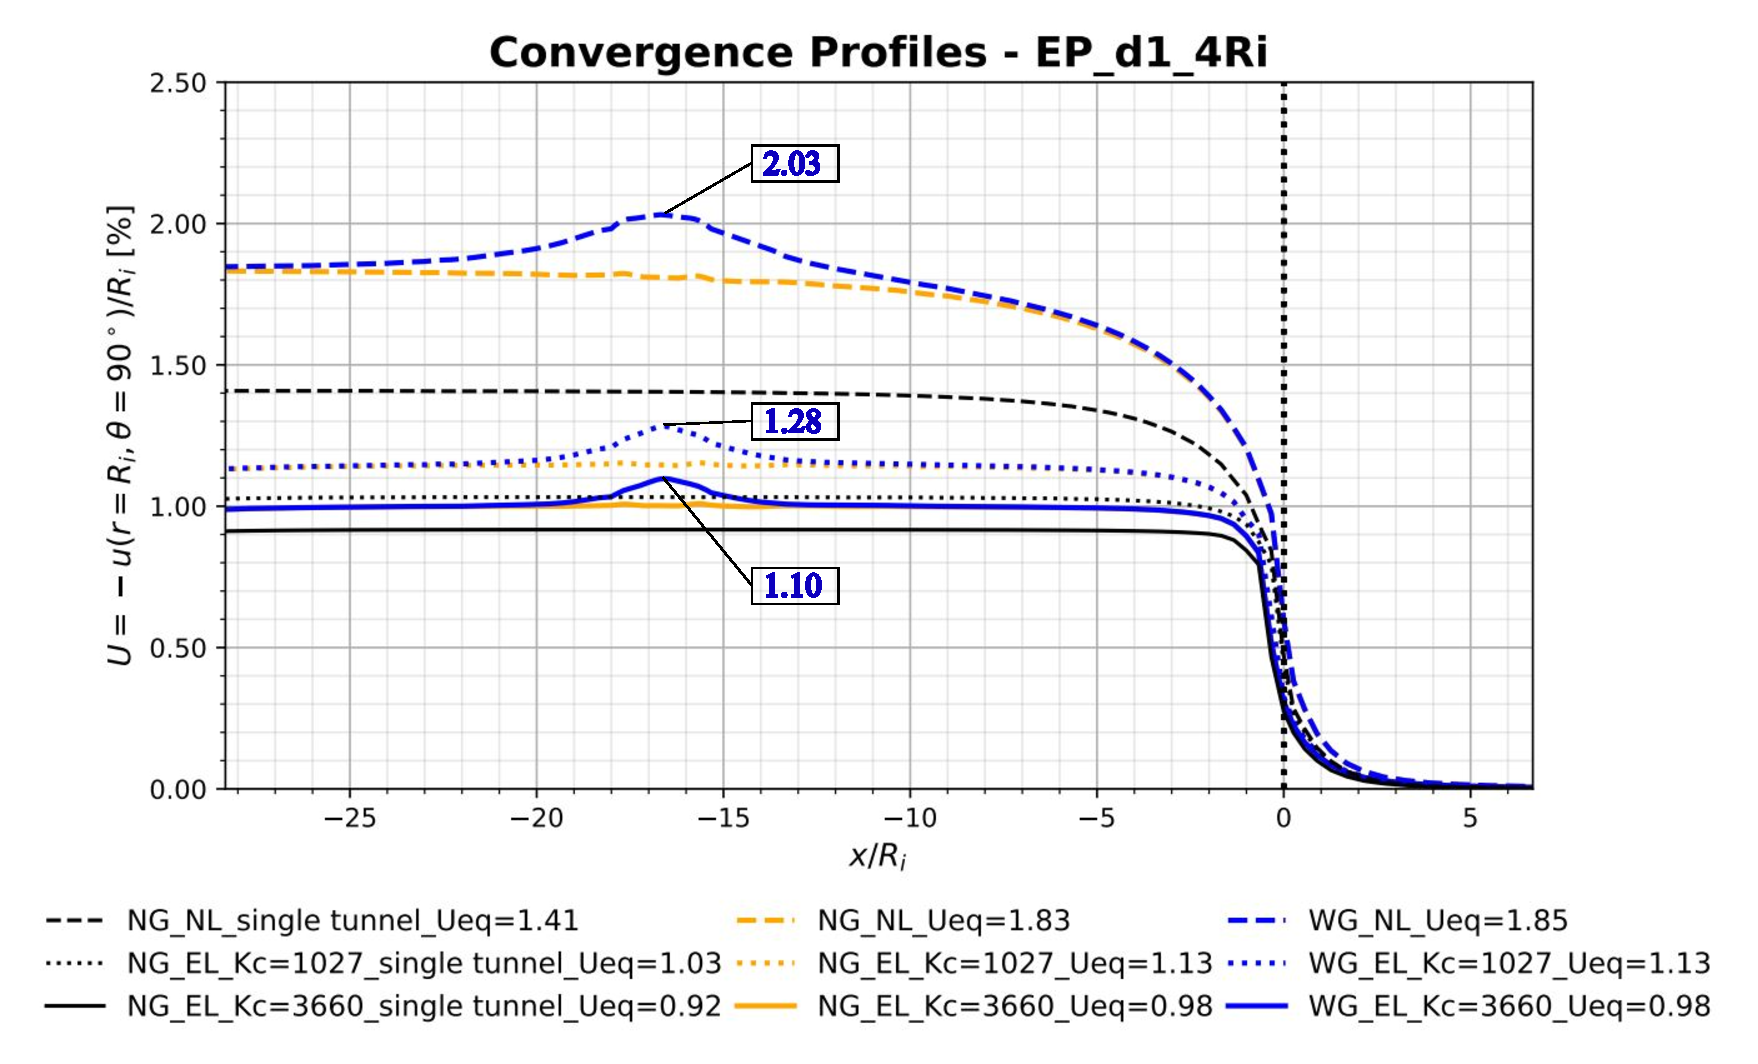
\includegraphics[scale=0.5]{Convergence Profiles - EP_d1_4Ri.pdf}
	\caption{Convergence Profiles - elastoplastic rock mass (EP) without lining (NL) with a highly stiff elastic lining ($K_c = 3660$ MPa) and a moderately stiff elastic lining ($K_c = 1027$ MPa), without (NG) and with gallery (WG) for $d_1 = 4R_i$}
	\label{EP_d1_4Ri}
\end{figure}
\FloatBarrier
For the single tunnel, a high stiffness lining (black solid line) decreases convergence by approximately 35\% compared to the unlined model (black dashed line). Conversely, a moderately stiff lining (black dotted line) increases convergence by 12\% compared to the rigid lining. 

When $d_1 = 16R_i$ between the twin tunnels (blue and yellow lines), the results of $U_{eq}$ are similar to the isolated tunnel (black line). However, with a distance reduced to $d_1 = 4R_i$, the interaction between the tunnels becomes significant. A smaller $d_1$, the high stiffness lining (solid yellow and blue lines) can restrict convergence by up to 46\% of the unlined (dashed yellow and blue lines) convergence. A moderate stiffness lining (dotted lines) leads to an increase of up to 16\% in convergence compared to the high stiffness lining (solid lines).

When comparing results between twin lined tunnels with spacings of $16R_i$ and $4R_i$, differences of 6\% with high stiffness lining (solid yellow and blue lines), 10\% with moderate stiffness lining (dotted yellow and blue lines), and 30\% without lining (dashed yellow and blue lines) are observed. These results show the direct impact of lining stiffness and the distance between twin tunnels on $U_{eq}$ convergence.

When analyzing the convergence $U_{peak}$ at the point where the gallery meets the longitudinal tunnel, there is an increase of 16\% when using an moderate stiffness elastic lining (dotted blue line) compared to a high stiffness lining (solid blue line). However, when analyzing the difference between the $U_{eq}$ and $U_{peak}$, there is a difference of up to 12\% for the high stiffness elastic lining (solid blue line to $4R_i$ and $16R_i$) and up to 13\% for the moderate stiffness elastic lining (dotted blue line to $4R_i$ and $16R_i$) for $d_1=4R_i$.

Applying the same type of previously analysis, we examine the elasto-plastic-viscoplastic model for the rock mass (EPVP), considering the presence of a viscoelastic lining (VEL) (Figs.~\ref{EPVP_VEL_d1_16Ri} and ~\ref{EPVP_VEL_d1_4Ri}). This analysis aims to comprehend the influence of the lining's stiffness, particularly when the twin tunnels are nearby. The results reveal that, once again, the convergence profile under these conditions, with a distance of $16R_i$ between the tunnels, closely resembles that of an isolated tunnel. Differences are on the order of 1.8\% for a moderately stiff lining and 0.8\% for a highly stiff lining.
\begin{figure}[h!]
	\centering
	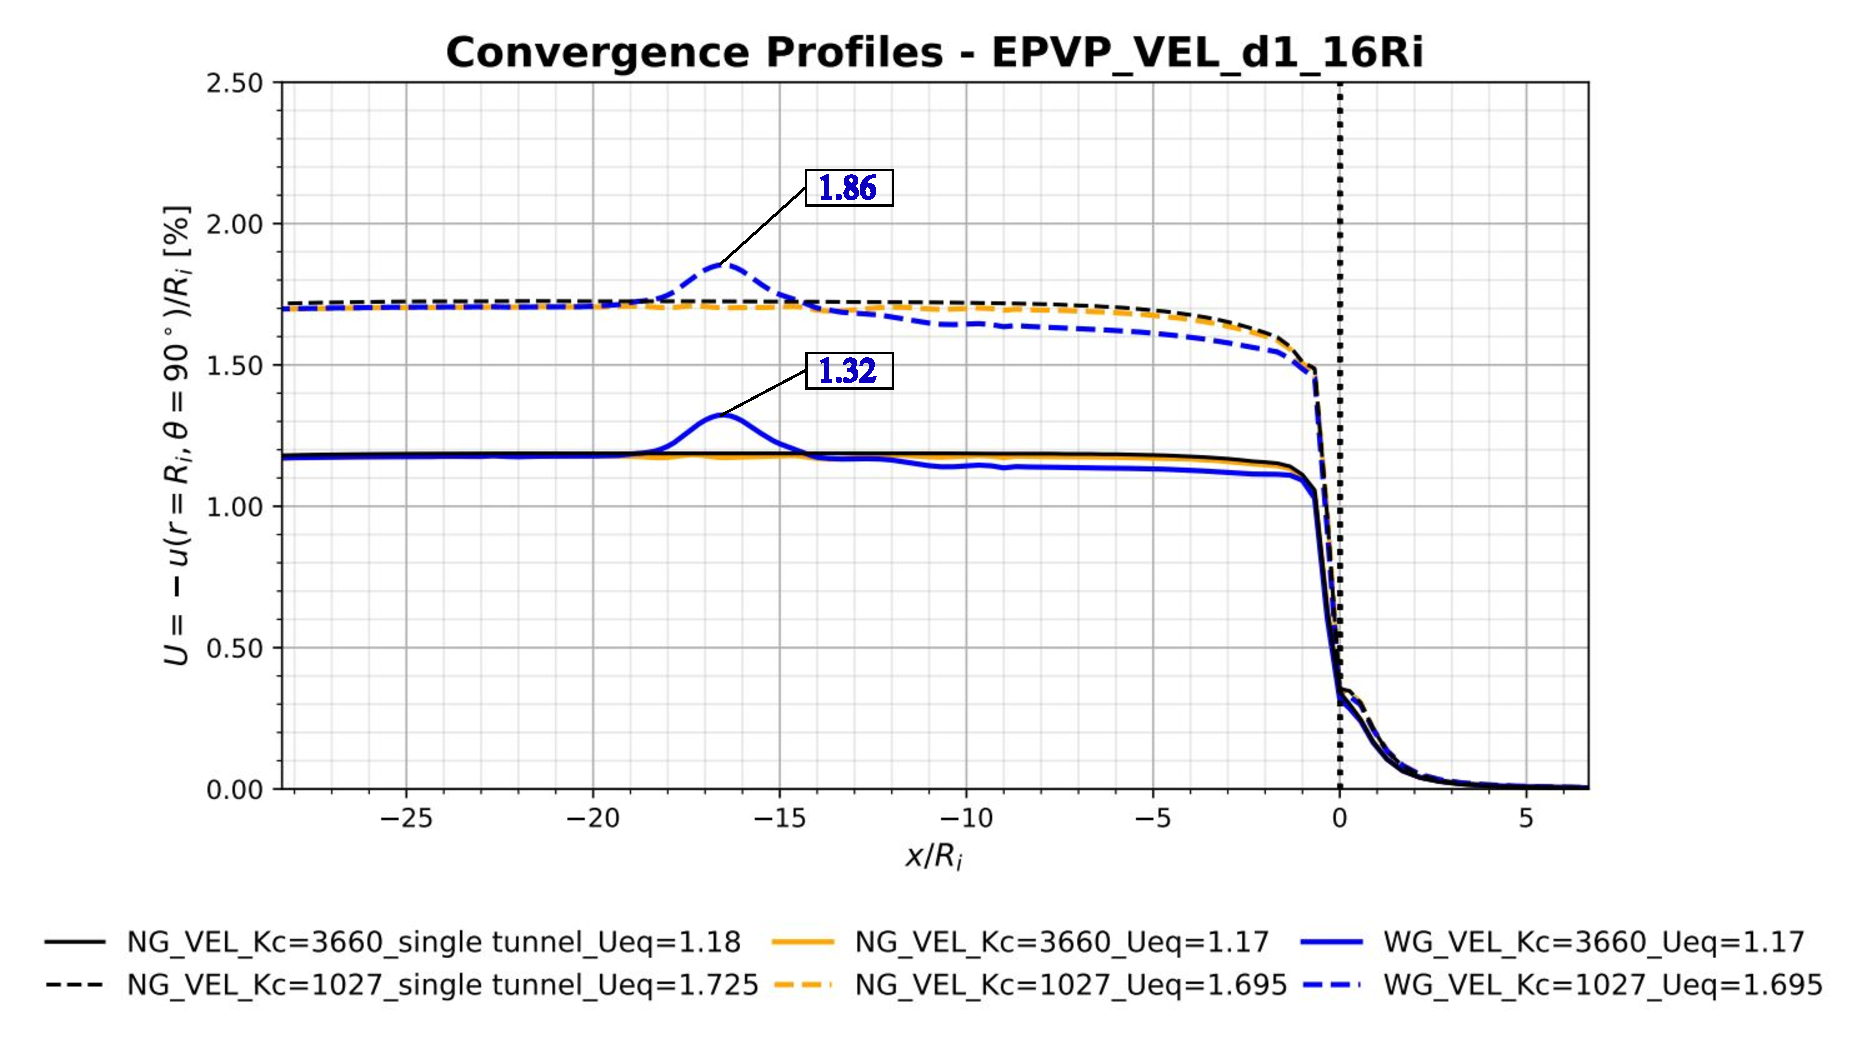
\includegraphics[scale=0.5]{Convergence Profiles - EPVP_VEL_d1_16Ri.pdf}
	\caption{Convergence Profiles - elasto-plastic-viscoplastic rock mass (EPVP) with a highly stiff viscoelastic lining ($K_c = 3660$ MPa) and a moderately stiff viscoelastic lining ($K_c = 1027$ MPa), without (NG) and with gallery (WG) for $d_1 = 16R_i$}
	\label{EPVP_VEL_d1_16Ri}
\end{figure}
\FloatBarrier
\begin{figure}[h!]
	\centering
	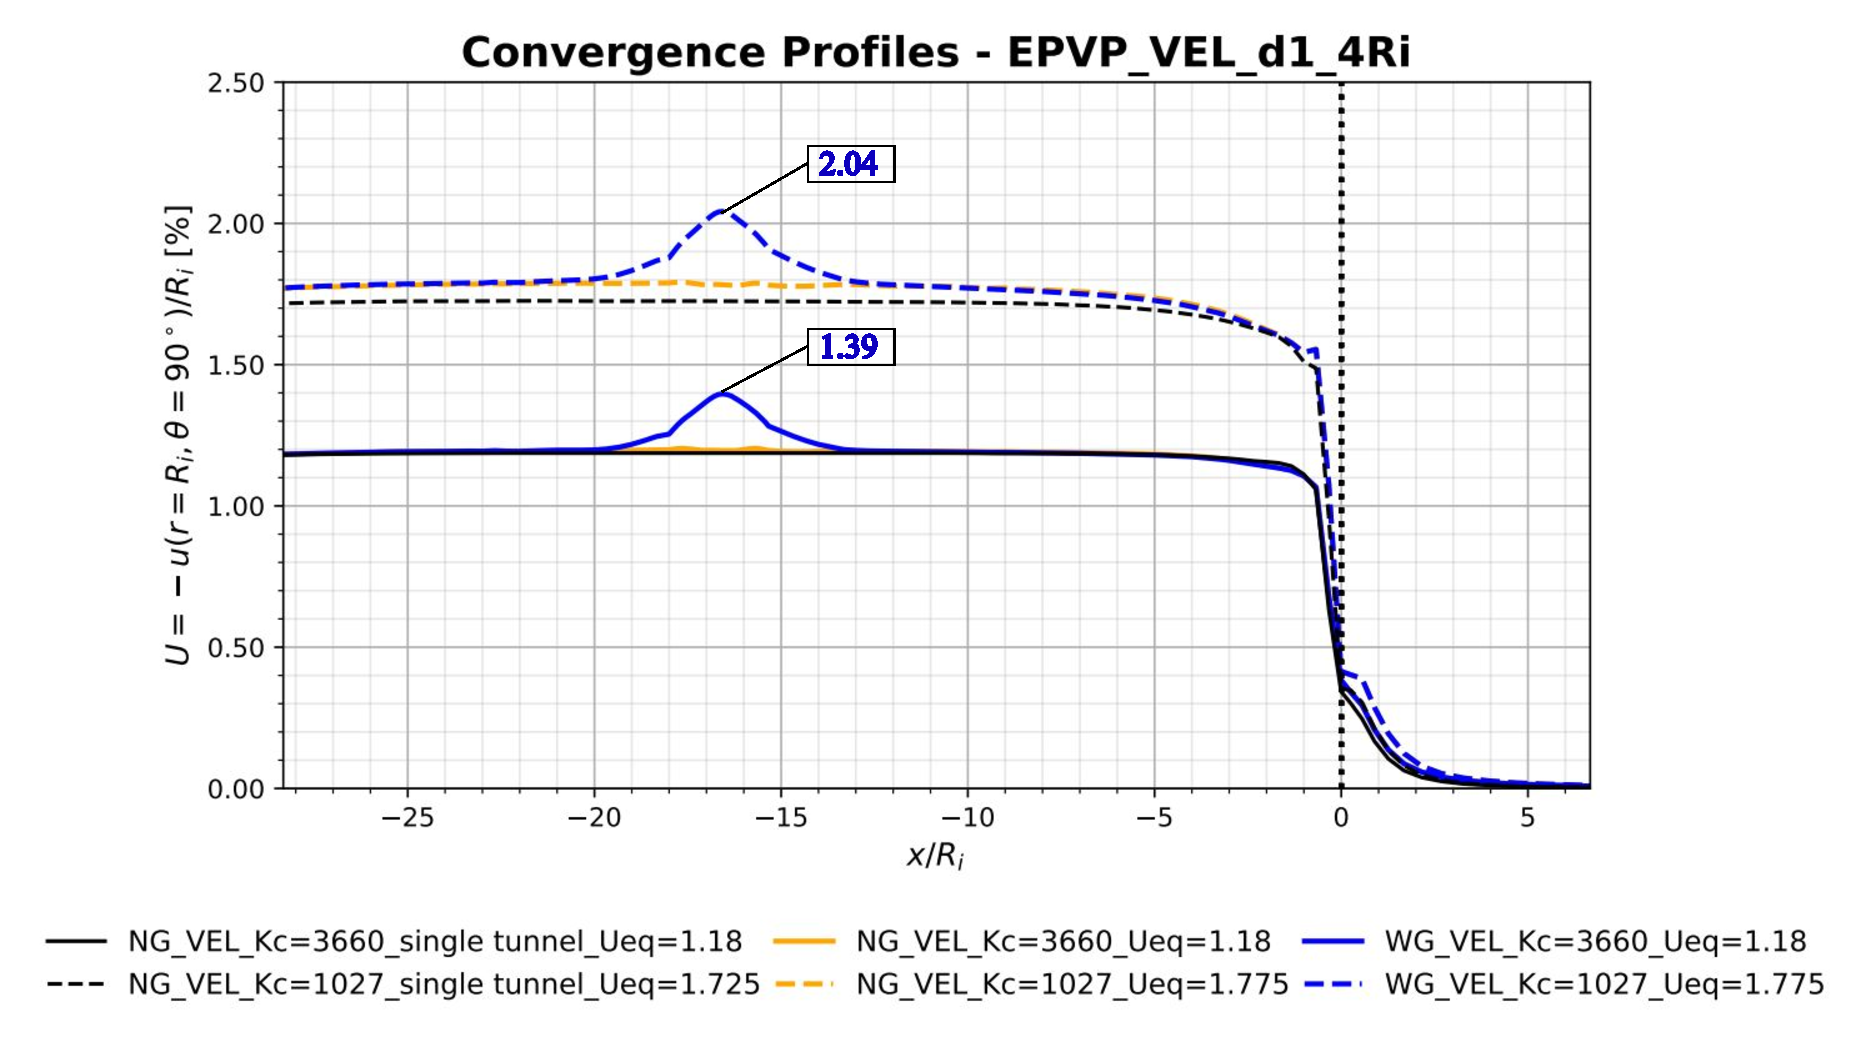
\includegraphics[scale=0.5]{Convergence Profiles - EPVP_VEL_d1_4Ri.pdf}
	\caption{Convergence Profiles - elasto-plastic-viscoplastic rock mass (EPVP) with a highly stiff viscoelastic lining ($K_c = 3660$ MPa) and a moderately stiff viscoelastic lining ($K_c = 1027$ MPa), without (NG) and with gallery (WG) for $d_1 = 4R_i$}
	\label{EPVP_VEL_d1_4Ri}
\end{figure}
\FloatBarrier
In the case of $d_1=4R_i$, when a high stiffness lining is applied (blue and yellow solid lines), there is practically no difference compared to the isolated tunnel (black solid line). This occurs because the high rigidity of the lining blocks convergence in the interaction between the tunnels. However, when using a moderately stiff lining (blue and yellow dashed lines), there is a difference of approximately 3\% in the convergence $U_{eq}$ compared to the single tunnel (black dashed line).

When comparing the results for $d_1 = 16R_i$ and $4R_i$, considering each lining separately, there is a difference of 0.8\% when there is a high stiffness lining (solid yellow and blue lines to $16R_i$ and $4R_i$) and 4.8\% for a moderate stiffness lining (dashed yellow and blue lines to $16R_i$ and $4R_i$). Thus, once again, the importance of the stiffness of the lining when associated with the distance between the twin tunnels.

When analyzing the convergence $U_{peak}$ at the point where the gallery meets the longitudinal tunnel, there is an increase of 47\% for $d_1=4R_i$ when using an moderate stiffness lining (dashed blue line) compared to a high stiffness lining (solid blue line). However, when analyzing the difference between the $U_{eq}$ and $U_{peak}$, there is a difference of up to 18\% for the high stiffness elastic lining (solid blue line) and up to 15\% for the moderate stiffness lining (dashed blue line) for $d_1=4R_i$.

The following results (Figs.~\ref{EPVP_EL_VEL_d1_16Ri} and ~\ref{EPVP_EL_VEL_d1_4Ri}) compare the elastic (EL) and viscoelastic (VEL) lining with high and moderate stiffness, considering the elastoplastic-viscoplastic (EPVP) model for the rock mass. 
\begin{figure}[h!]
	\centering
	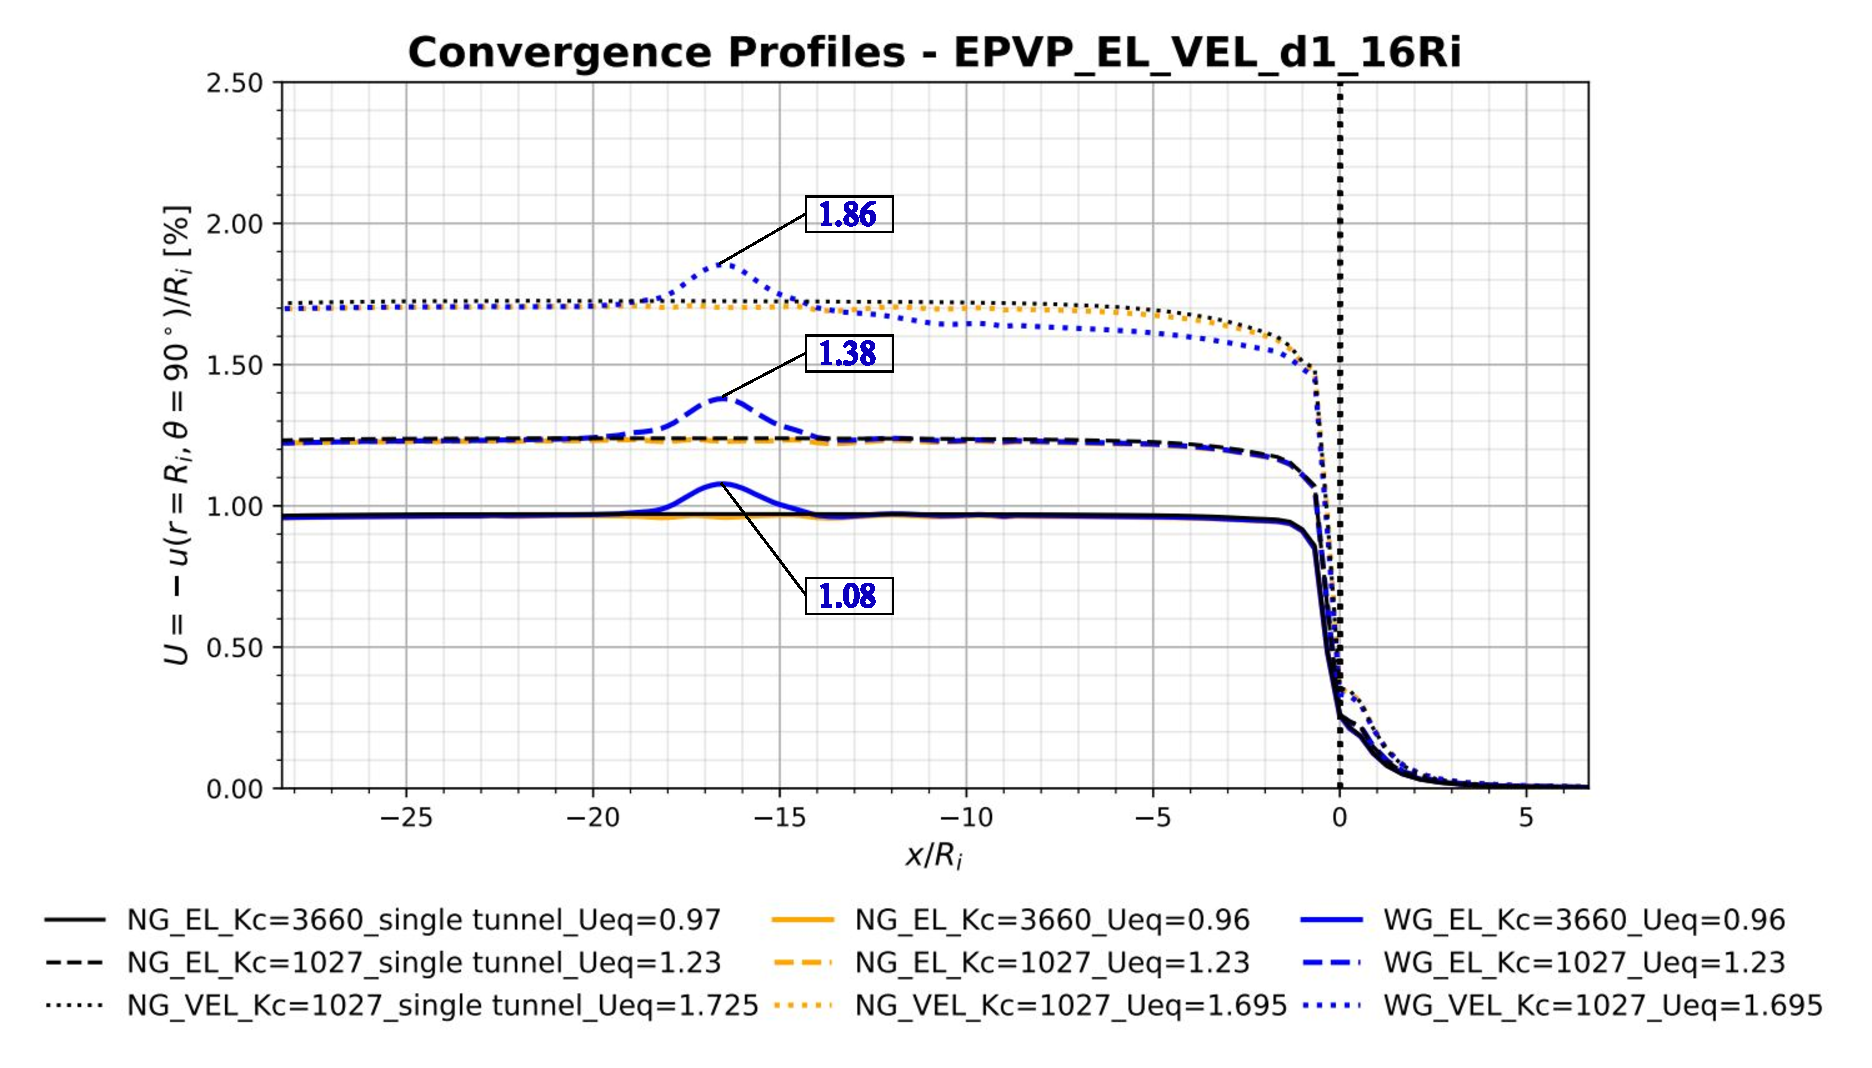
\includegraphics[scale=0.5]{Convergence Profiles - EPVP_EL_VEL_d1_16Ri.pdf}
	\caption{Convergence Profiles - elasto-plastic-viscoplastic rock mass (EPVP) without lining (NL) with a highly stiff ($K_c = 3660$ MPa) and a moderately stiff ($K_c = 1027$ MPa) elastic (EL) and viscoelastic (VEL) lining, without (NG) and with gallery (WG) for $d_1 = 16R_i$}
	\label{EPVP_EL_VEL_d1_16Ri}
\end{figure}
\FloatBarrier
\begin{figure}[h!]
	\centering
	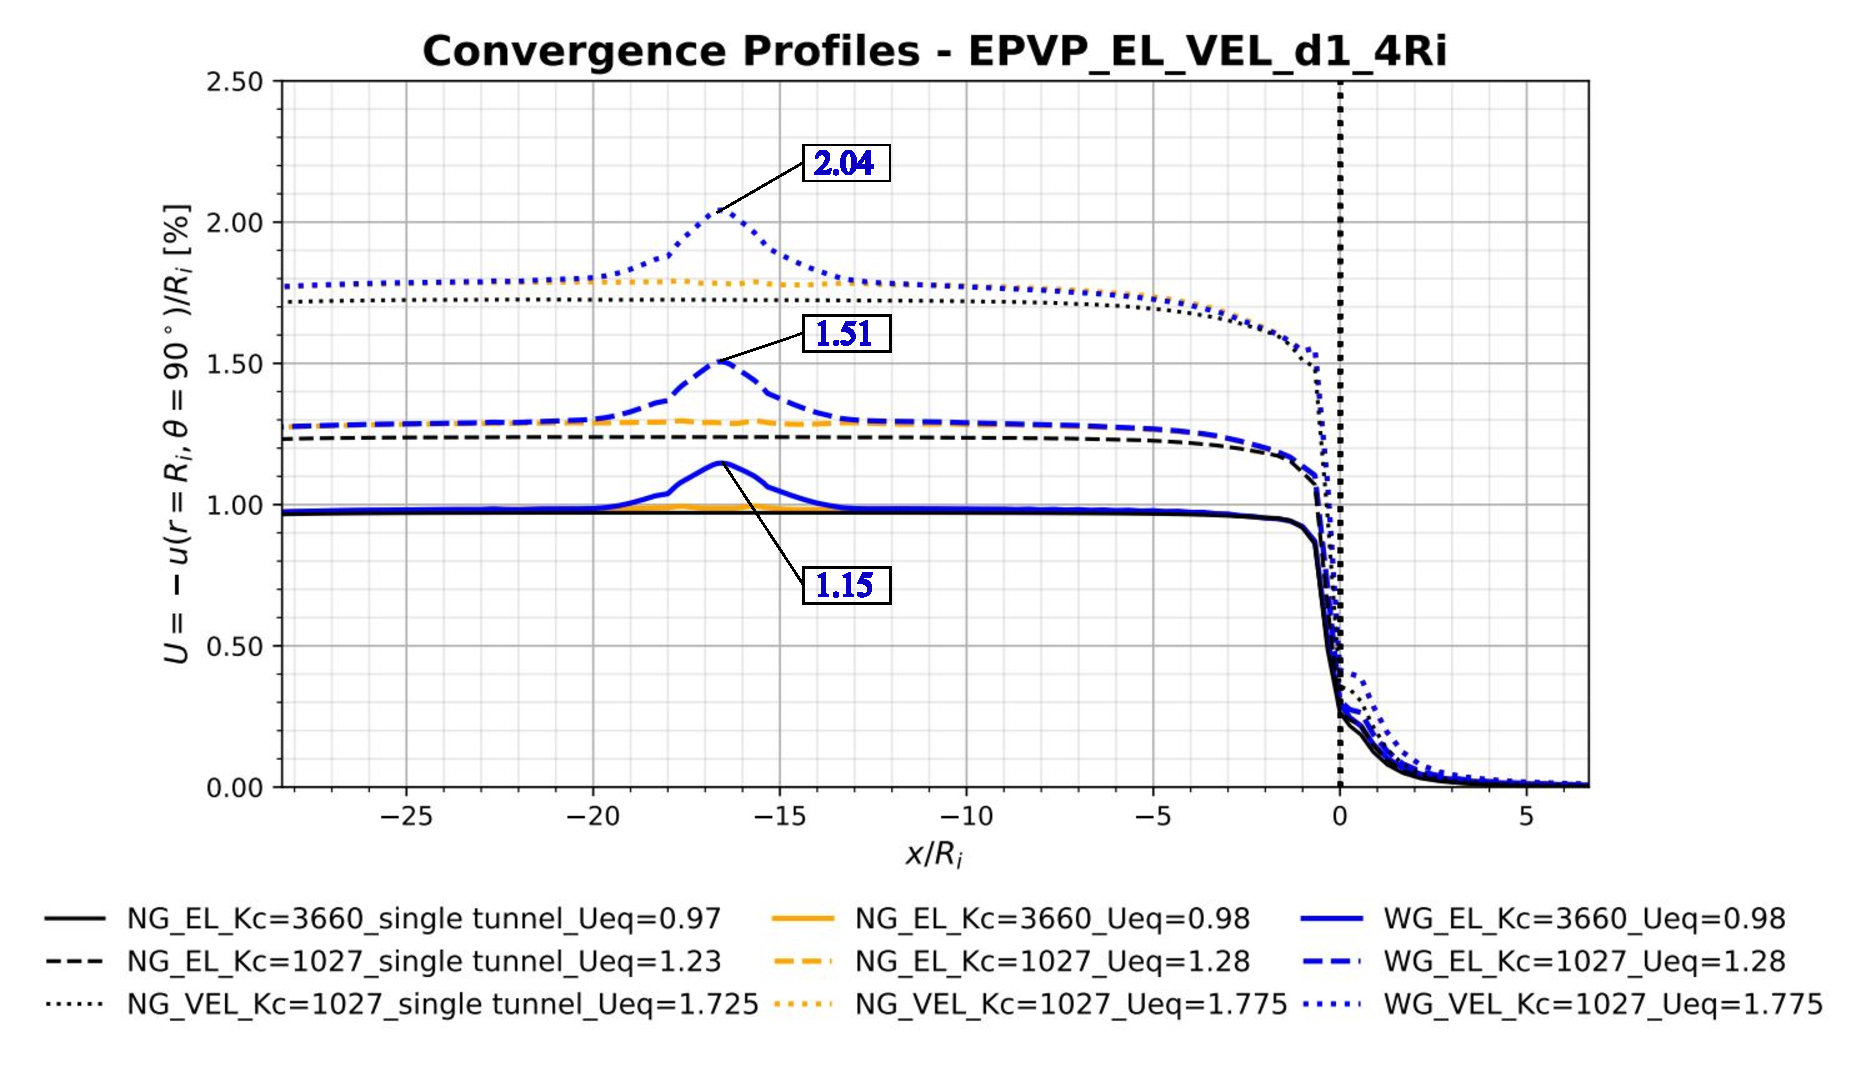
\includegraphics[scale=0.5]{Convergence Profiles - EPVP_EL_VEL_d1_4Ri.pdf}
	\caption{Convergence Profiles - elasto-plastic-viscoplastic rock mass (EPVP) without lining (NL) with a highly stiff ($K_c = 3660$ MPa) and a moderately stiff ($K_c = 1027$ MPa) elastic (EL) and viscoelastic (VEL) lining, without (NG) and with gallery (WG) for $d_1 = 4R_i$}
	\label{EPVP_EL_VEL_d1_4Ri}
\end{figure}
\FloatBarrier
For $d_1=16R_i$, the significant difference in $U_{eq}$ compared to the isolated tunnel (dotted black line) occurs when considering the moderate stiffness viscoelastic lining (dotted blue line), with approximately 1.8\%. In contrast, for $d_1=4R_i$, the differences are 4\% and 3\% for the elastic (dashed lines) and viscoelastic (dotted lines) linings with moderate stiffness, respectively.

When adopting the high stiffness elastic lining as a reference (solid lines), for $d_1 = 16R_i$, the differences increase to 27\% and 78\% when comparing the elastic (dashed lines) and viscoelastic (dotted lines) lining with moderate stiffness, respectively, and to 31\% and 81\% in the case of $d_1=4R_i$.

When analyzing the convergence at the peak $U_{peak}$, which corresponds to the point where the gallery meets the longitudinal tunnel, and using the value of the high stiffness elastic lining (solid lines) as the reference, an increase of up to 31\% and 77\% is observed for $d_1=4R_i$ when using the elastic (dashed lines) and viscoelastic (dotted lines) linings of moderate stiffness, respectively.

However, when analyzing the difference between the $U_{eq}$ and $U_{peak}$, there is a difference of up to 18\% for the moderate stiffness elastic lining (dashed blue line) and up to 15\% for the moderate stiffness viscoelastic lining (dotted blue line) for $d_1=4R_i$.

Finally, Fig.~\ref{EP_EPVP_NG_LT_single tunnel} a comparison between the lining elastic and viscoelastic, considering high and moderate stiffness, and between the elastoplastic and elastoplastic-viscoelastic models for the rock mass. We adopt the condition of an isolated tunnel, starting from the reference value of the elastoplastic rock mass with high stiffness elastic lining. 
\begin{figure}[h!]
	\centering
	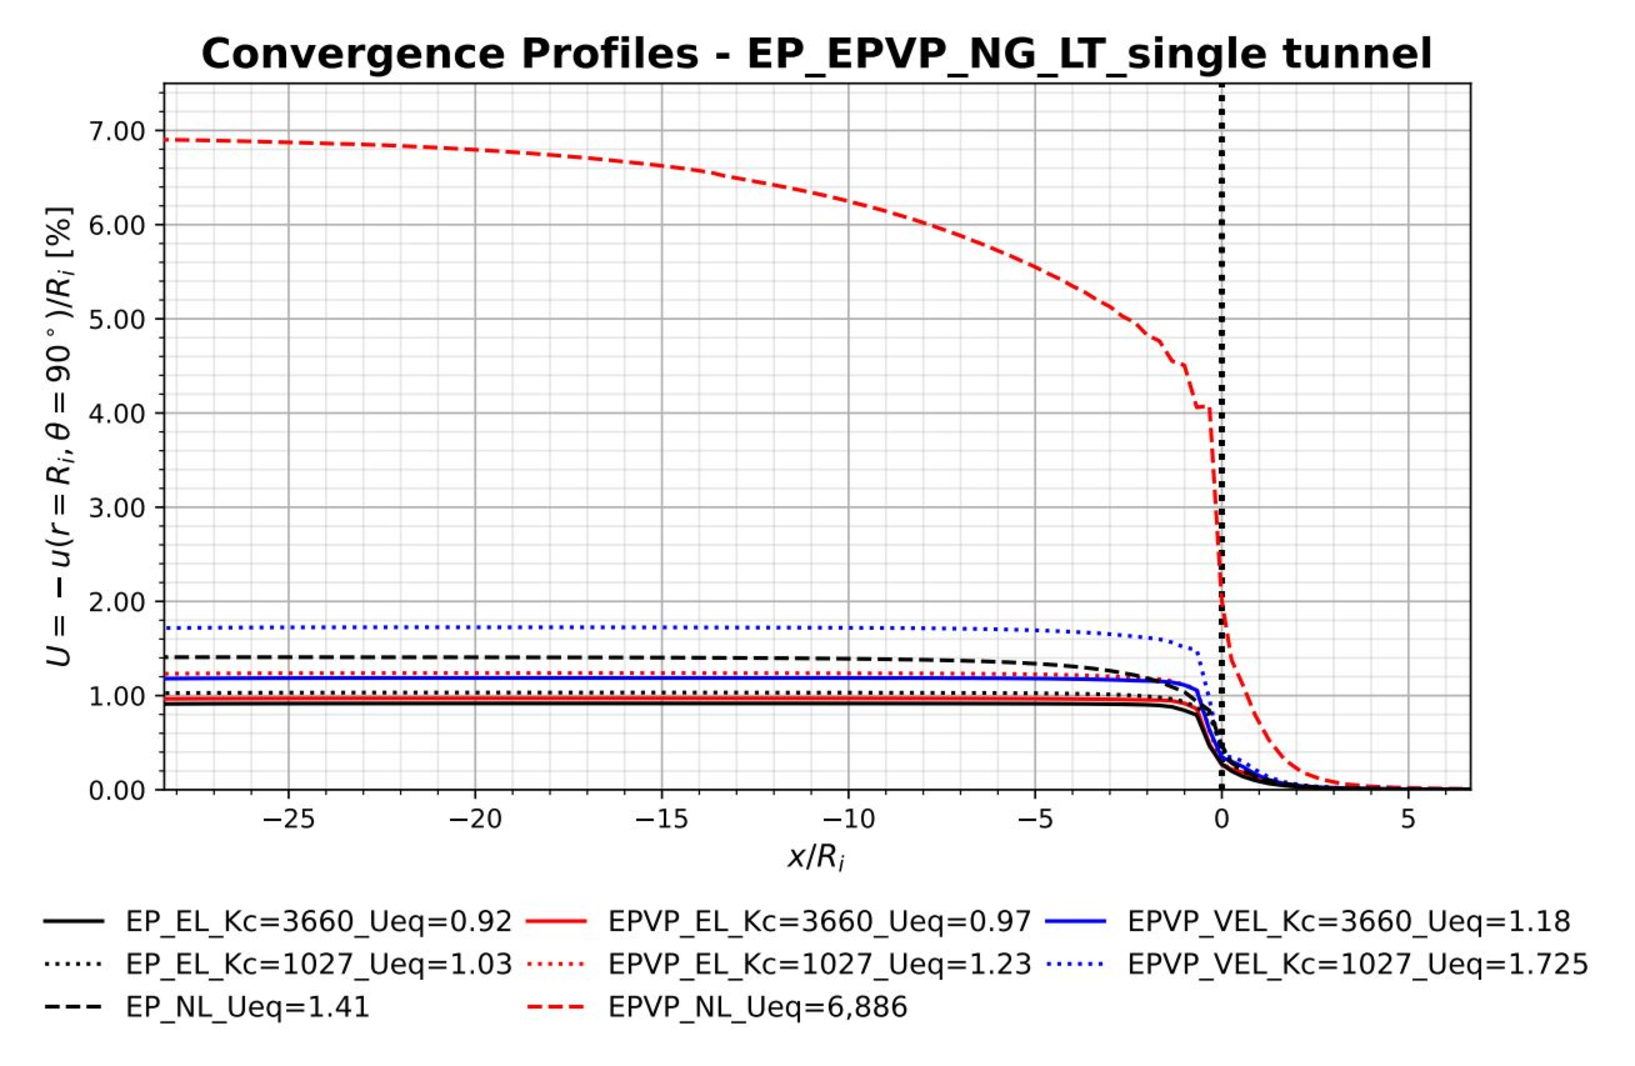
\includegraphics[scale=0.5]{Convergence Profiles - EP_EPVP_NG_LT_single tunnel.pdf}
	\caption{Convergence Profiles - single tunnel with elastoplastic (EP) and elasto-plastic-viscoplastic rock mass (EPVP), without lining (NL) with a highly stiff ($K_c = 3660$ MPa) and a moderately stiff ($K_c = 1027$ MPa) elastic (EL) and viscoelastic (VEL) lining}
	\label{EP_EPVP_NG_LT_single tunnel}
\end{figure}
\FloatBarrier
Taking as a reference the elastoplastic model with a highly stiffness elastic lining (solid black line) we observed a difference of 12\% and 53.5\%, respectively, in the cases of the elastoplastic rock mass with an elastic lining of moderate stiffness (dotted black) and without a lining (dashed black line). We also identified a difference of 5.5\%, 33.5\%, and 748\% when using the elastoplastic-viscoplastic model for the rock mass with an elastic lining of high stiffness (solid red line), moderate stiffness (dotted red line), and no lining (dashed red line). In addition, we found a difference of 28\% and 87.5\% when comparing the elastoplastic-viscoplastic model for the rock mass and the viscoelastic model for the high stiffness (solid blue line) and moderate stiffness lining (dotted blue line), respectively.

\section{Conclusions}\label{}

The fundamental role of the stiffness of the concrete lining in the convergence profile of twin tunnels is understood from the analyses. Depending on the value of this stiffness, it is possible to condition the restriction of viscous effects that tend to manifest over time after the completion of the excavation process.

Additionally, the effect of the interaction between longitudinal tunnels is notable when considering proximity, with significant influence from a distance of 4 radii. However, in many cases, this effect may be subtle or almost imperceptible due to the presence of a highly rigid lining.

In models considering the viscosity of the rock mass, the time factor plays a significant role in convergence. In this scenario, when excavating the gallery with $d_1 = 16R_i$, the portion of the tunnel already excavated remains subject to viscous effects for a more extended period compared to other distances. In any case, when $d_1 = 4R_i$, the proximity interaction between twin tunnels, along with viscous effects over time, results in a higher value compared to cases where $d_1 = 16R_i$ and $8R_i$.

Another important observation related to EPVP-EL and EPVP-VEL models concerns the possible ovalization of the section over time, concerning the analyzed reference point on the section perimeter (in the crown). Instead of following the logic of following the closing direction of the section, it may undergo some negative displacement in the long term. The result, for the same observation point, is a convergence value that in the short term may indicate section closure but in the long term may indicate the opposite.

Another crucial observation regarding EPVP-EL and EPVP-VEL models pertains to the potential ovalization of the section over time, particularly concerning the analyzed reference point on the section perimeter (in the crown). Instead of conforming to the expected logic of closing in the section's direction, it might experience negative displacement in the long term. Consequently, for the same observation point, the convergence value may initially suggest section closure in the short-term but indicate the opposite in the long-term.

Concerning the EPVP-VEL model, specifically with distances of 16 and 8 radii between twin tunnels, we observe that Ueq in the section ahead of the gallery region is slightly smaller than Ueq in the section preceding the gallery. This variation in the convergence profile results from the shorter exposure time to viscous effects in the portion excavated later than the transverse gallery. Therefore, during the gallery excavation process, the portion of the longitudinal tunnel already excavated experiences viscous effects until completing the gallery excavation. 

However, concerning the existence of a transverse gallery and adopting the constitutive parameters while considering the presence of lining, its influence is highly localized, spanning approximately four radii on each side from its axis. Consequently, there is no significant impact on the remaining convergence profile of the tunnels, except for the model with viscoelastic lining, where lower convergences occur after the gallery. 

%% To print the credit authorship contribution details
%\printcredits
%
%%% Loading bibliography style file
%%\bibliographystyle{model1-num-names}
\bibliographystyle{cas-model2-names}
%
%% Loading bibliography database
\bibliography{cas-refs}
%
%% Biography
%\bio{}
%% Here goes the biography details.
%\endbio
%
%\bio{pic1}
%% Here goes the biography details.
%\endbio

\end{document}

